% !TeX encoding = UTF-8
%% \textbf{重庆大学}通用毕业论文\LaTeXe{}模板
%%% 使用前请先阅读使用文档和用户协议,内有详细介绍。Happy Texing! :)
%% =======================================================
\documentclass%
	[type=bachelor, bilinguallist=apart,]{cquthesis}%
% 可用选项:
% type=[bachelor|master|doctor],      % 必选,毕业论文类型,以下项目不填时为默认
% liberalformat,                      % 可选,仅适用本科生,使用文学类论文标题格式,默认未打开
% proffesionalmaster=[true|false],    % 可选,仅适用研究生,是(true)否(false)专业硕士,默认为否
% printmode=[oneside|twoside|auto],	  % 可选,论文打印方式,默认采用auto按页数要求自动判定
% openany,|openright,                 % 可选,双面打印时每章的第一页仅右页开启,默认右页开启(openright)
% bilinguallist=[off|combined|apart], % 可选,图录表录等分别按双语题注混编(combined),分开编录(apart),默认关(off)
% blindtrail,                         % 可选,盲审模式,开启后封面姓名和致谢部分会隐藏,详情请参阅用户文档,默认关
% draft,                              % 写作期间可选,不渲染图片,关闭外围功能,加快预览速度,默认未开启

% 请在cquthesis.sty文件中定义其他会用到的宏包和自己的变量
% 这样可以防止main.tex太过臃肿。
\usepackage{cquthesis}
\usepackage{listings} % 附录中添加代码块
\usepackage{xcolor}
\lstset{
	columns=fixed,       
	numbers=left,                                        % 在左侧显示行号
	frame=none,                                          % 不显示背景边框
	backgroundcolor=\color[RGB]{245,245,244},            % 设定背景颜色
	numberstyle=\footnotesize\color{darkgray},           % 设定行号格式
	stringstyle=\rmfamily\slshape\color[RGB]{128,0,0},   % 设置字符串格式
	showstringspaces=false,                              % 不显示字符串中的空格
	language=sas,                                        % 设置语言
}



% 定义所有的图片文件在 figures 子目录下
\graphicspath{{figures/}}

%*** 写作时,使用这个命令只渲染你想查看的部分,提升工作效率,定稿时注释掉整行
%\includeonly{contents/experiment,contents/analysis,}

\begin{document}

\cqusetup{
%	************	注意	************
%	* 1. \cqusetup{}中不能出现全空的行,如果需要全空行请在行首注释
%	* 2. 不需要的配置信息可以放心地坐视不理、留空、删除或注释(都不会有影响)
%	*
%	********************************
% ===================
%	论文的中英文题目
% ===================
  ctitle = {基于大数据下二叉树定价实现},
  etitle = {Binomial Tree Pricing Practice Based on Big Data},
% ===================
% 作者部分的信息
% \secretize{}为盲审标记点,在打开盲审开关时内容会自动被替换为***输出,盲审开关默认关闭
% ===================
  cauthor = \secretize{赵赞豪},	% 你的姓名,以下每项都以英文逗号结束
  eauthor = \secretize{Zanhao~Zhao},	% 姓名拼音,~代表不会断行的空格
  studentid = \secretize{11501040136},	% 仅本科生,学号
  csupervisor = \secretize{肖枝洪~~教授},	% 导师的姓名
  esupervisor = \secretize{{Prof.~Zhihong Xiao}},	% 导师的姓名拼音
  % cassistsupervisor = \secretize{}, % 本科生可选,助理指导教师姓名,不用时请留空为{}
  % cextrasupervisor = \secretize{}, % 本科生可选,校外指导教师姓名,不用时请留空为{}
  % eassistsupervisor = \secretize{}, % 本科生可选,助理指导教师或/和校外指导教师姓名拼音,不用时请留空为{}
  cpsupervisor = \secretize{肖枝洪~~教授}, % 仅专硕,兼职导师姓名
  epsupervisor = \secretize{Prof.~Zhihong Xiao},	% 仅专硕,兼职导师姓名拼音
  cclass = 理学,	% 博士生和学硕填学科门类,学硕填学科类型
  edgree = {Mathematics and Applied Mathematics (Mathematical Finance) },	% 专硕填Professional Degree,其他按实情填写
% 提示:如果内容太长,可以用\zihao{}命令控制字号,作用范围:{}内
  cmajor = {\zihao{-4}数学与应用数学(数理金融)},	% 专硕不需填,填写专业名称
  emajor = Mathematics and Applied Mathematics (Mathematical Finance) , % % 专硕不需填,填写专业英文名称
% ===================
% 底部的学院名称和日期
% ===================
  cdepartment = 理学院,	%学院名称
  edepartment = College of Science ,	%学院英文名称
% ===================
% 封面的日期可以自动生成(注释掉时),也可以解除注释手动指定,例如:二〇一六年五月
% ===================
%	mycdate = {中文日期},
%	myedate = {Date in English},
}% End of \cqusetup
% ===================
%
% 论文的摘要
%
% ===================
%%%%%%%%%%%%%%%%%%%%%%%%%%%%%%%%%%%%%%%%%%%%%%%%%%%%
\begin{cabstract}	% 中文摘要
	本文档运用了\LaTeX{}进行编译生成文档。
	
	本文主要讲述基于大数据下的二叉树期权定价模型的实现方法、实现步骤、实现结果的展示。
	
	首先,本文讲述了期权的含义,以及传统期权定价中的二叉树模型、Black-Schools期权定价模型、蒙特卡罗期权定价模型。
	
	然后,本文接着讲述了基于大数据下的期权定价模型。
	
	再接着就是对三种传统期权定价模型的实现。在这里,主要运用SAS、R、Python这三种语言分别对传统期权定价下的二叉树模型、Black-Schools期权定价模型、蒙特卡罗期权定价模型进行实现。然后是对基于大数据下的期权定价模型进行实现。
	
	
	
	
	
  

\end{cabstract}
% 中文关键词,请使用英文逗号分隔:
\ckeywords{期权定价,二叉树,BS模型,蒙特卡罗,大数据}



%%%%%%%%%%%%%%%%%%%%%%%%%%%%%%%%%%%%%%%%%%%%%%%%%%%%

\begin{eabstract}	% 英文摘要
	
	English abstract(none).
	
	
\end{eabstract}
% 英文关键词,请使用英文逗号分隔,关键词内可以空格:
\ekeywords{bachelor, none}

% 封面和摘要配置完成

\makecover %%% 封面部分


\frontmatter %%%前置部分(封面后绪论前)

%% 摘要
\makeabstract

%% 目录,注意需要多次编译才能更新
\tableofcontents

%% 插图索引,可选,如不用可注释掉
\listoffigures
\listoffiguresEN

%% 表格索引,可选
\listoftables
\listoftablesEN

%% 公式索引,可选
\listofequations
\listofequationsEN

%% 符号对照表,可选
%% !TeX encoding = UTF-8
% 环境用两个长度参数,分别定义左边距以及词条和解释的水平距离,可自己调试以达美观(全去掉时默认:20mm,30mm)

% 主要符号对照表
\begin{denotation}[10mm][40mm]
	\item[CQU] 重庆大学(Chongqing University)的英文缩写
	\item[\LaTeX] 一个很棒的排版系统
	\item[\LaTeXe] 一个很棒的排版系统的最新稳定版
	\item[\XeTeX] \LaTeX{}的好兄弟,事实上他有很多个兄弟,但是这个兄弟对各种语言的支持能力都很强
	\item[CTeX宏集] 成套的中文\LaTeX{}解决方案,由一帮天才们开发
	\item[\ce{H2SO4}] 硫酸
	\item[$ e^{\pi{}i}+1=0$] 一个集自然界五大常数一体的炫酷方程
	\item[\ce{2H2 + O2 -> 2H2O}] 一个昂贵的生成生命之源的方程式
\end{denotation}

\endinput



\mainmatter %%% 主体部分(绪论开始,结论为止)
%* 子文件的多少和内容由你决定(最好以章为单位),基本原则是提速预览、脉络清晰、管理容易。

%% 正文绪论
\chapter{绪论}













%% 传统定价模型和基于大数据下定价模型
\chapter{传统期权定价模型}

\section{二叉树定价模型}


\section{Black-Schools期权定价模型}


\section{蒙特卡罗期权定价模型}




\chapter{基于大数据下的期权定价模型}

\section{决策树定价模型}


%% 传统定价模型的实现和基于大数据下定价模型的实现


\chapter{传统期权定价模型实现}
	在金融衍生品的定价中,二叉树模型、Black-Schools模型和蒙特卡罗方法都受到了很大的应用。


%%%%%%%%%%%%%%%% 二叉树定价模型
\section{二叉树定价模型实现}

\subsection{R实现二叉树定价模型}
	使用CRR的二叉树多期期权定价模型,可以通过R软件中通过自带的函数CRRBinomialTreeOption来实现。本案例主要是实现两个功能:第一,期权定价计算;第二,二叉树定价结果显示,R代码详见附录。
	
	模型参数结果设置如下,见Parameters中的输出结果。在函数中,TypeFlag的取值有:ce、ca、pe、pa,其中c与p分别表示看涨与看跌期权,e与a分别表示欧式与美式期权。与此同时,令S=100,X=110,Time=0.5,r=0.05,b=0.05,sigma=0.2,n=3。
	
	本文中运用的R版本是3.5.3,二叉树模型运行的结果如下图所示:
	
	\begin{figure}[htb] % use float package if you want it here
		\centering
		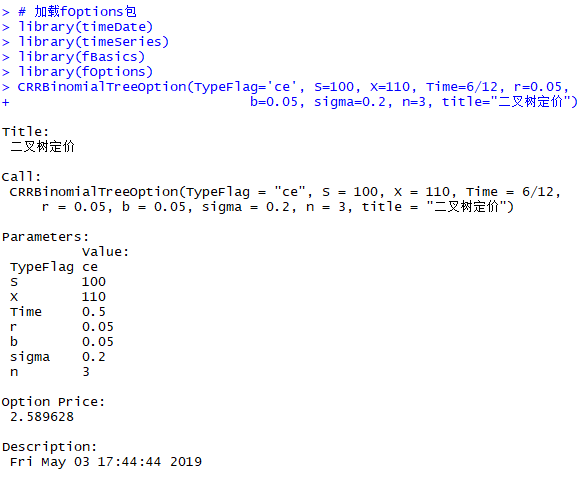
\includegraphics[height=8cm]{Rerchashu.png}
		\bicaption{使用R进行二叉树定价}{Binomial tree pricing by using R}
		\label{fig:xfig1}
	\end{figure}
	
	在上图中,可以知道二叉树定价的价格是2.589628。
	
	在R的fOptions这个包中,有一个GBSOption函数可以间接的求出Black-Schools模型的定价结果,下面给出BS模型的定价结果,用来做比较。(这里令S=100,X=110,Time=0.5,r=0.05,b=0.05,sigma=0.2)具体结果如下图所示:
	
	\begin{figure}[htb] % use float package if you want it here
		\centering
		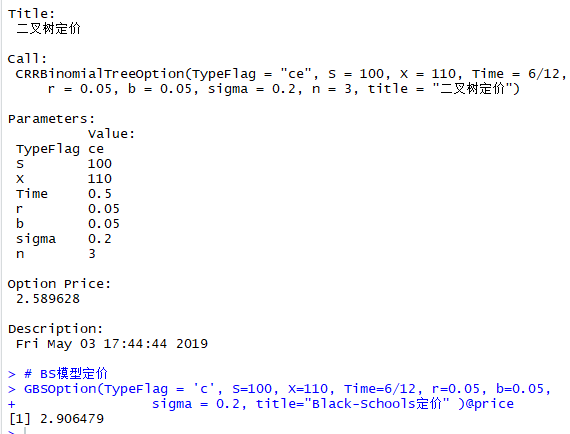
\includegraphics[height=5cm]{BSR.png}
		\bicaption{BS模型验证二叉树模型结果}{ }
		\label{fig:xfig1}
	\end{figure}

	从上述的结果中个,可以知道二叉树定价的价格为2.589628,但是Black-Schools期权定价模型的价格为2.906479,两者价格相差不大。
	下面的例子开始绘制二叉树定价的树状图。由于二叉树定价的过程不太好表述,所以可以绘制一张图来清晰的表达二叉树的结果。具体的图像如下所示:
	
	\begin{figure}[htb] % use float package if you want it here
		\centering
		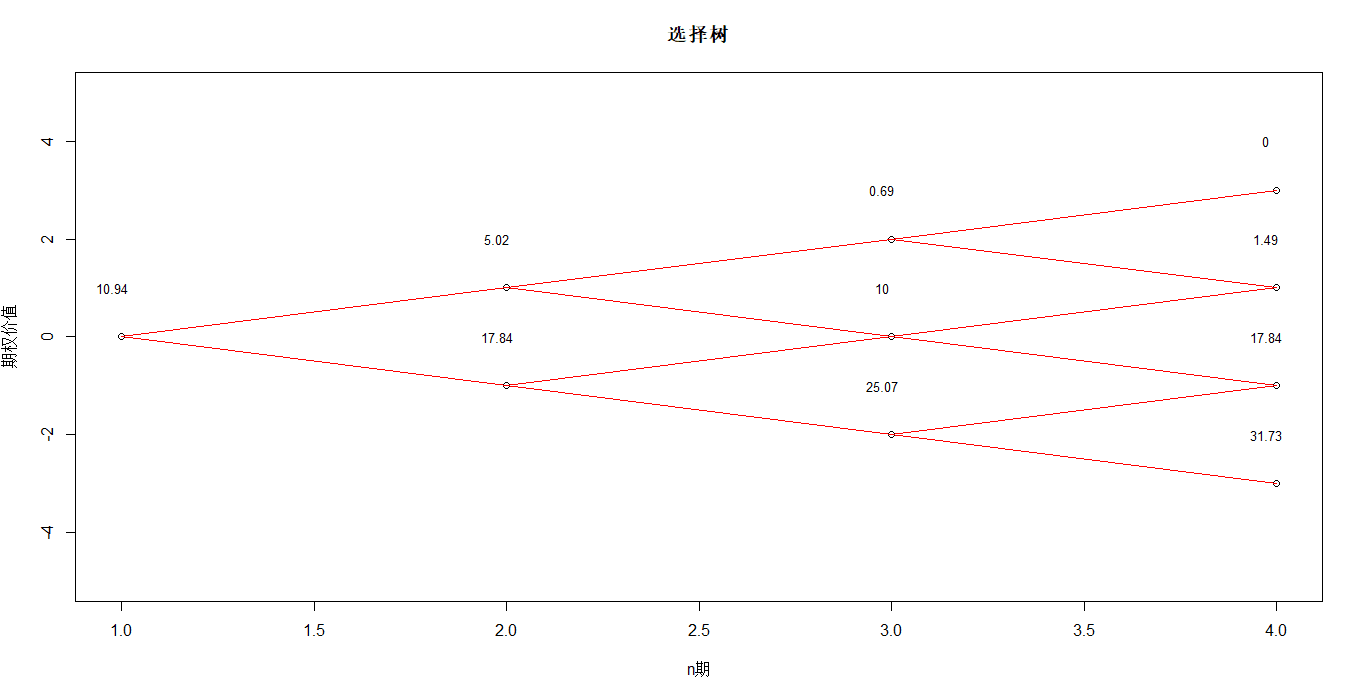
\includegraphics[height=5cm]{Rhuizhi1.png}
		\bicaption{R实现二叉树定价模型的结果绘制}{ }
		\label{fig:xfig1}
	\end{figure}

	从上图,可以清晰地看出二叉树期权定价的结果。

	当然,R也能绘制出20期期权定价的结果:
	
	\begin{figure}[htb] % use float package if you want it here
		\centering
		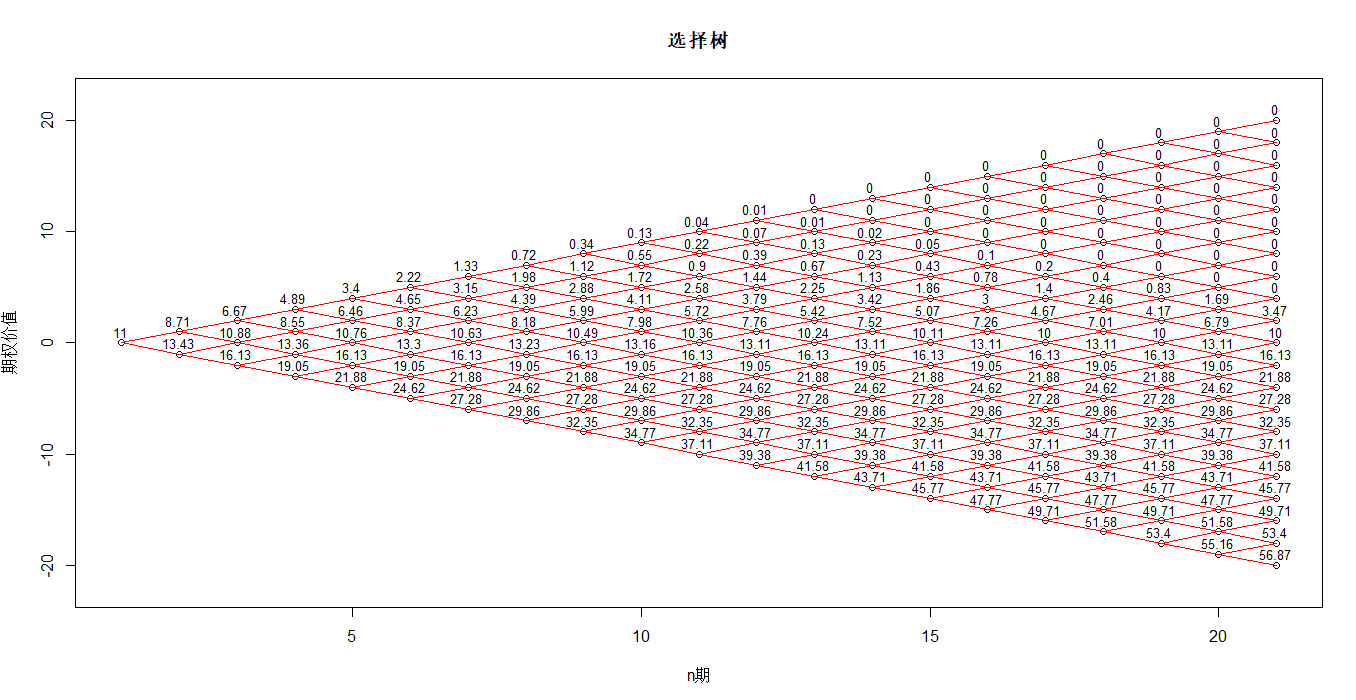
\includegraphics[height=7cm]{R20tu.png}
		\bicaption{20期期权定价结果图}{ }
		\label{fig:xfig1}
	\end{figure}
	
	
	\begin{figure}[htb] % use float package if you want it here
		\centering
		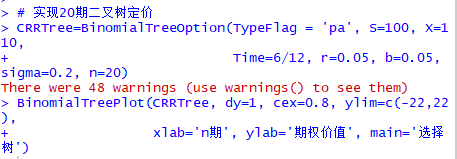
\includegraphics[height=5cm]{R20code.png}
		\bicaption{绘制20期期权定价代码}{ }
		\label{fig:xfig1}
	\end{figure}




\subsection{SAS实现二叉树定价模型}
	当然,SAS语言也可以像R语言一样,有着自己的二叉树期权定价函数。但是,也可以用SAS程序进行10期期权的二叉树定价,具体的实现过程如下各图:
	
	在下图中,可以知道:第0期股价S$_{0}$为100,$u=1.1,d=0.9$,各期无风险利率为$ r_{f}=0.05 $,期权的执行价格为$X=100$。
	
	首先输出的是SAS语言进行二叉树定价实现图。图中左边显示的是SAS的资源管理器和结果,中间显示的是日志窗口,最右边显示的是增强型编辑器窗口。
	
	\begin{figure}[htb] % use float package if you want it here
		\centering
		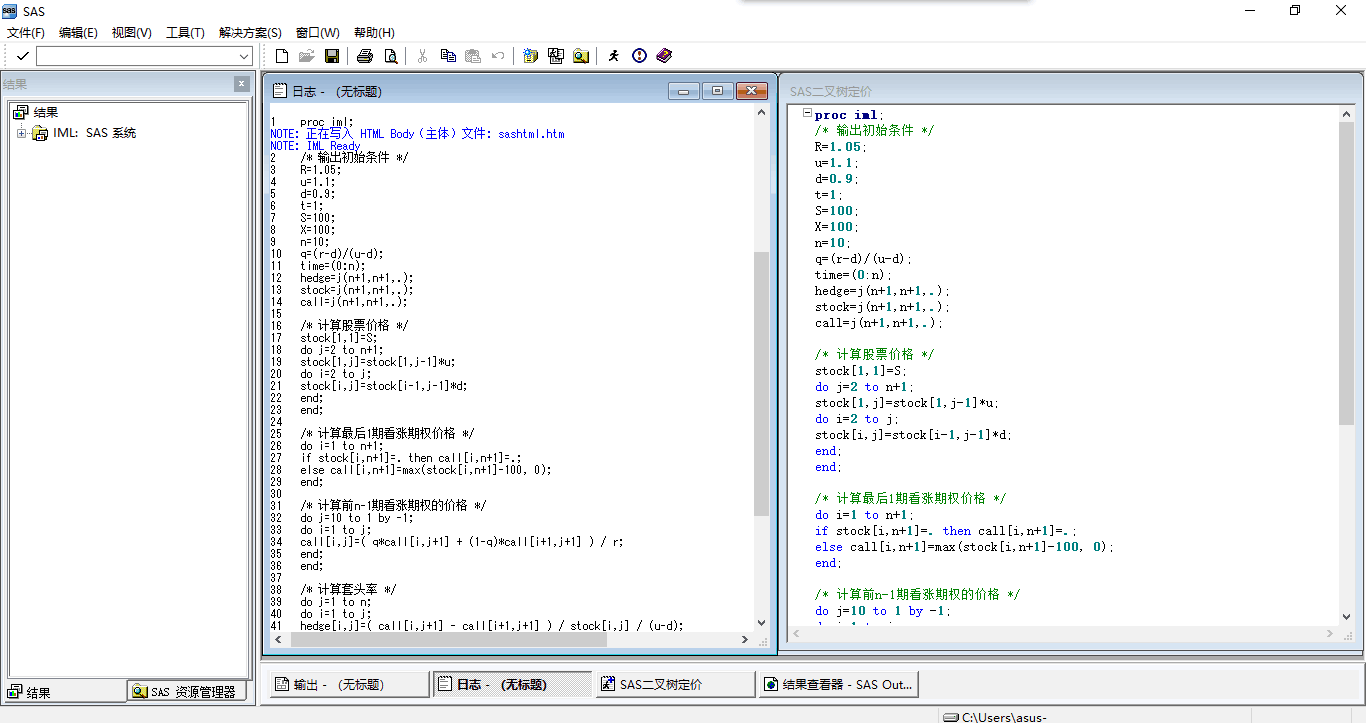
\includegraphics[height=5cm]{SASerchashu1.png}
		\bicaption{SAS语言进行二叉树定价实现}{ }
		\label{fig:xfig1}
	\end{figure}
	
	接下来输出的是10期模型各期期末股票价格变动图。
	
	\begin{figure}[htb] % use float package if you want it here
		\centering
		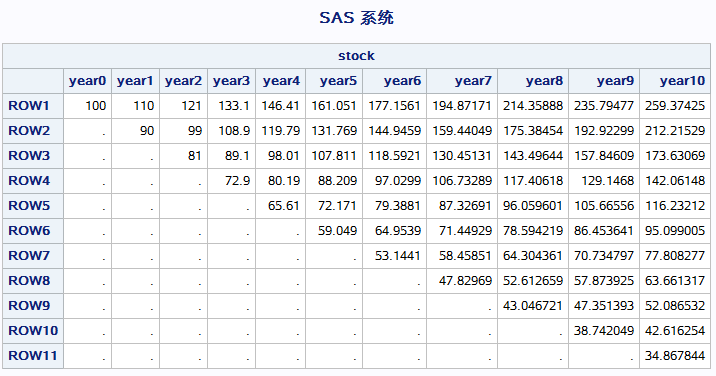
\includegraphics[height=5cm]{SASerchashu2.png}
		\bicaption{10期二叉树模型各期期末股票价格变动图}{ }
		\label{fig:xfig1}
	\end{figure}
	
	接下来输出的是10期模型各期期末的期权价格计算图。
	
	\begin{figure}[htb] % use float package if you want it here
		\centering
		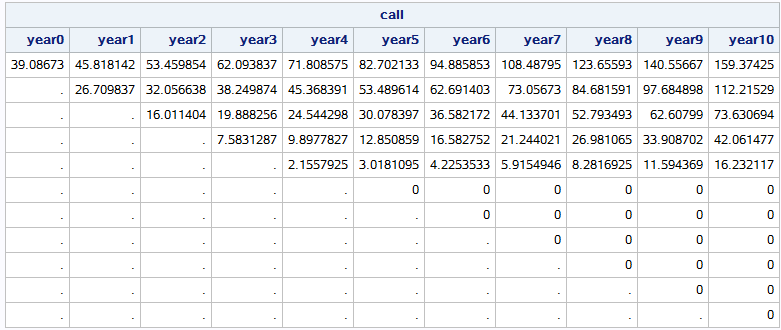
\includegraphics[height=5cm]{SASerchashu3.png}
		\bicaption{10期二叉树模型各期期末期权价格变动图}{ }
		\label{fig:xfig1}
	\end{figure}
	
	接下来输出的是:
	
	\begin{figure}[htb] % use float package if you want it here
		\centering
		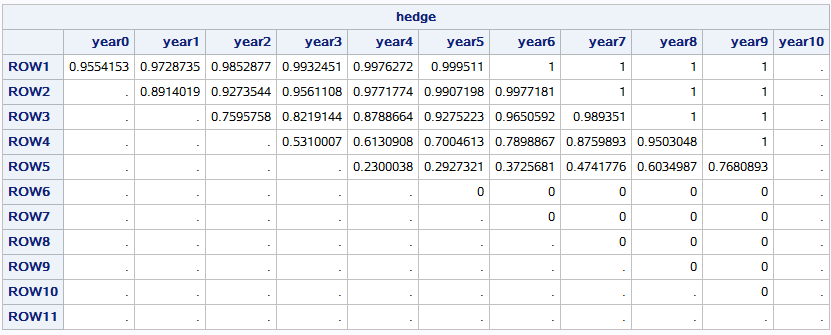
\includegraphics[height=5cm]{SASerchashu4.png}
		\bicaption{10期二叉树模型 }{ }
		\label{fig:xfig1}
	\end{figure}
	
%%	强制换页
\clearpage	

\subsection{Python实现二叉树模型的准备工作}
	二叉树期权定价模型中,标的资产价格在每一时间节点都有上升和下降的两种可能性。由于期权是标的资产的衍生工具,因此二叉树期权定价模型基于离散时间跟踪标的资产,它可以为欧式期权、美式期权,以及百慕大期权定价。
	
\subsubsection{编写StockOption类}
	利用Python运行多种期权定价方法前,先编写一个StockOption类,相当于SAS的封装宏一样,存储好股票期权的通用计算方法。将代码存为StockOption.py文件放在当前的工作目录,等待调用即可。即下图所示:
	
	\begin{figure}[htb] % use float package if you want it here
		\centering
		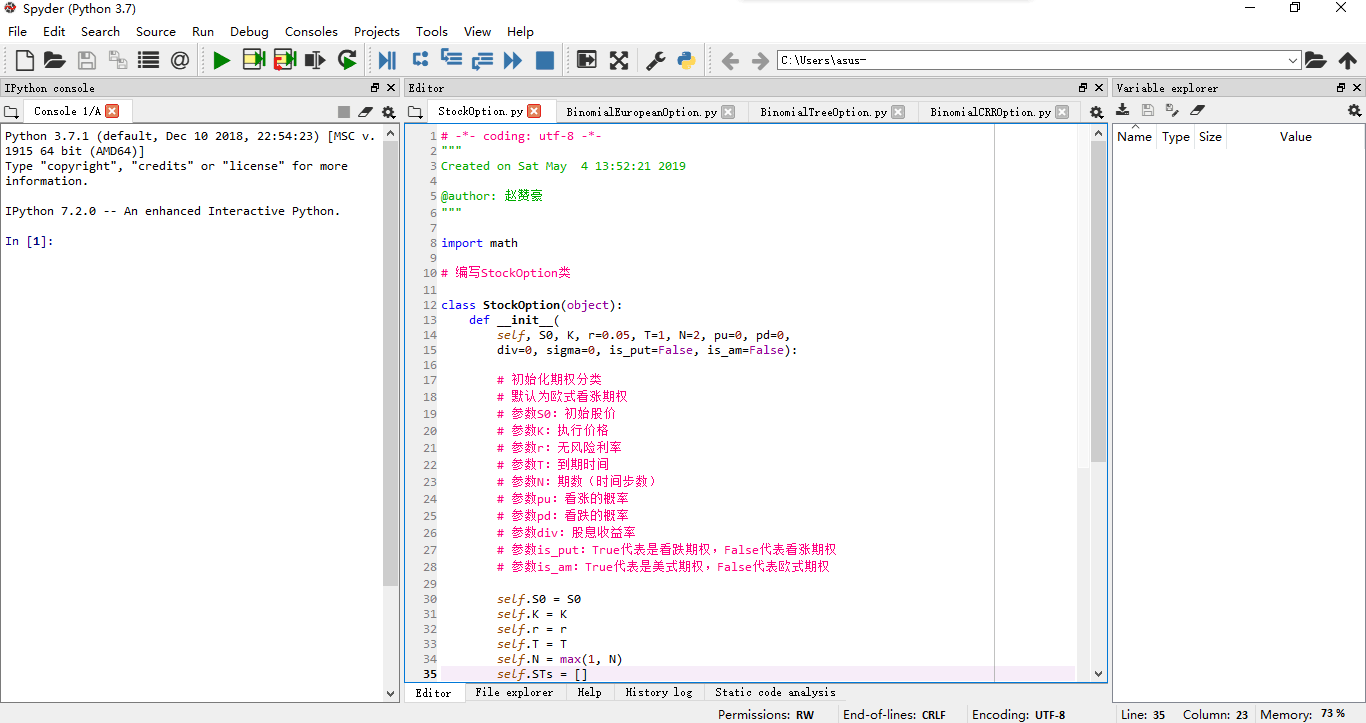
\includegraphics[height=5cm]{StockOption.png}
		\bicaption{StockOption类的编写 }{ }
		\label{fig:xfig1}
	\end{figure}

	标的资产的当前价格、行权价格、无风险利率、到期时间和时间步长的取值是期权定价所需的通用属性。其中,params变量是一个字典对象,接受模型所需的附加信息。时间步长dt和贴现率df在运行定价程序时可以反复使用。
	
\subsubsection{编写BinomialEuropeanOption类}
	Python包含对欧式期权进行二叉树定价的BinomialEuropeanOption类,该类与StockOption类使用同一期权通用属性。
	
	BinomialEuropeanOption类的定价方法是解决此类问题的通用方法。该方法调用\_setup\_parameters\_建立所需的模型参数,再调用\_initialize\_stock\_price\_tree预测T期的股票价格。最后调用私有的方法\_\_begin\_tree\_traversal\_\_,初始化收益值数组并存储折现收益值,该方法将遍历二叉树至当前结点。收益树节点作为NumPy数组对象返回,其中欧式期权的当前价值出现在初始节点。
	
	\begin{figure}[htb] % use float package if you want it here
		\centering
		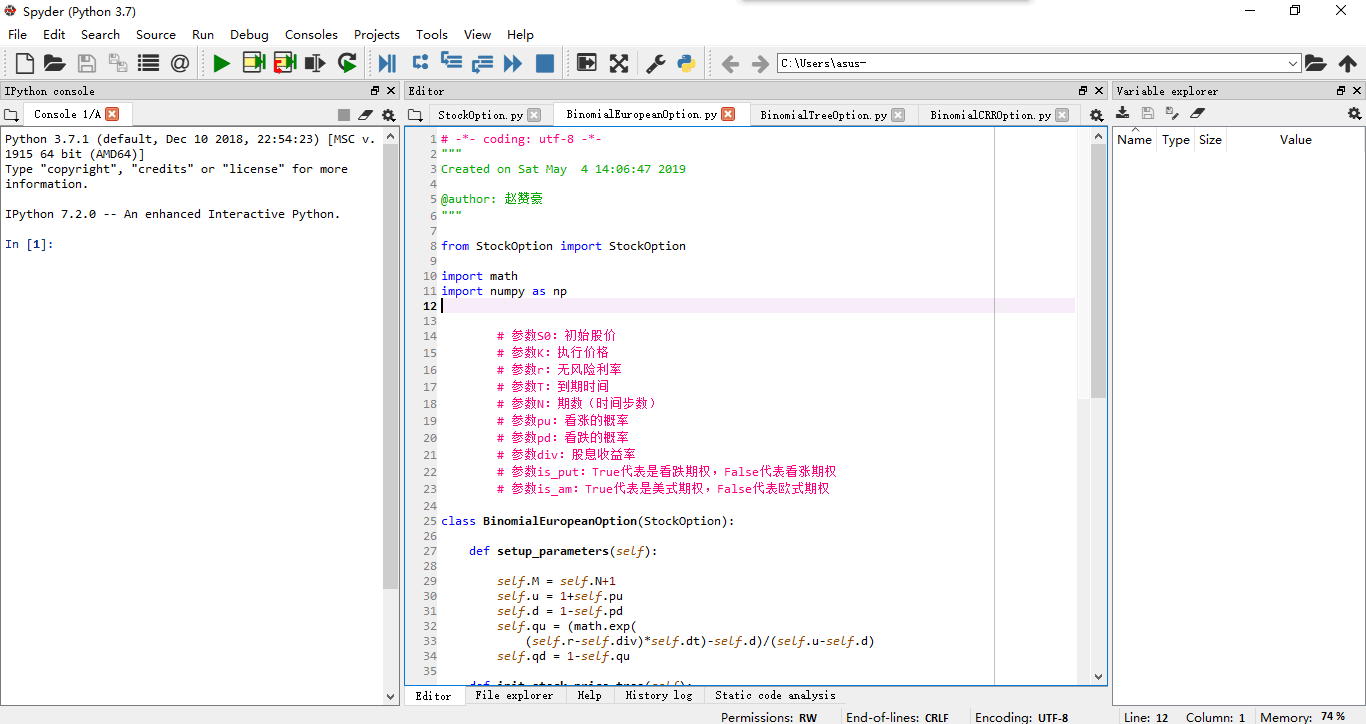
\includegraphics[height=5cm]{BinomialEuropeanOption.png}
		\bicaption{BinomialEuropeanOption类的编写 }{ }
		\label{fig:xfig1}
	\end{figure}

	需要注意的是,以双下划线开头的方法叫做私有方法,只能在同一类中访问。以单下划线开头的方法是受保护的方法,该方法可能被子类覆盖。不以下划线开头的方法为公共函数,可以从任何对象中使用。因为我曾经看过一段时间的Java,这和Java有些相似。
	
\subsubsection{编写BinomialTreeOption类}
	编写BinomialTreeOption类的主要目的是为了给美式期权定价。与欧式期权不同,美式期权可以在到期日前任意时间行权。用Python实现美式期权定价时,需要创建一个名为BinomialTreeOption的类。
	
	\begin{figure}[htb] % use float package if you want it here
		\centering
		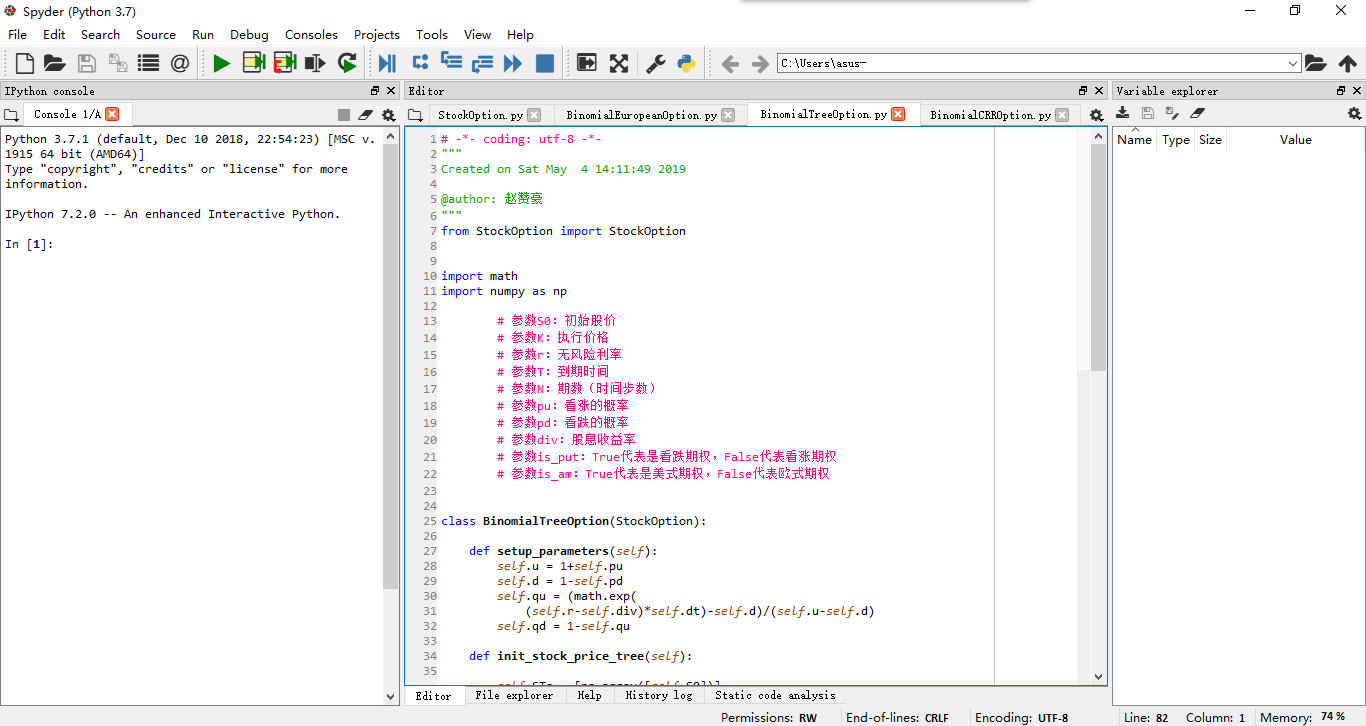
\includegraphics[height=5cm]{BinomialTreeOption.png}
		\bicaption{BinomialTreeOption类的编写 }{ }
		\label{fig:xfig1}
	\end{figure}

\subsubsection{编写BinomialCRROption类}
	创建一个BinomialCRROption类,可以为欧式期权和美式期权同时定价。
	
	\begin{figure}[htb] % use float package if you want it here
		\centering
		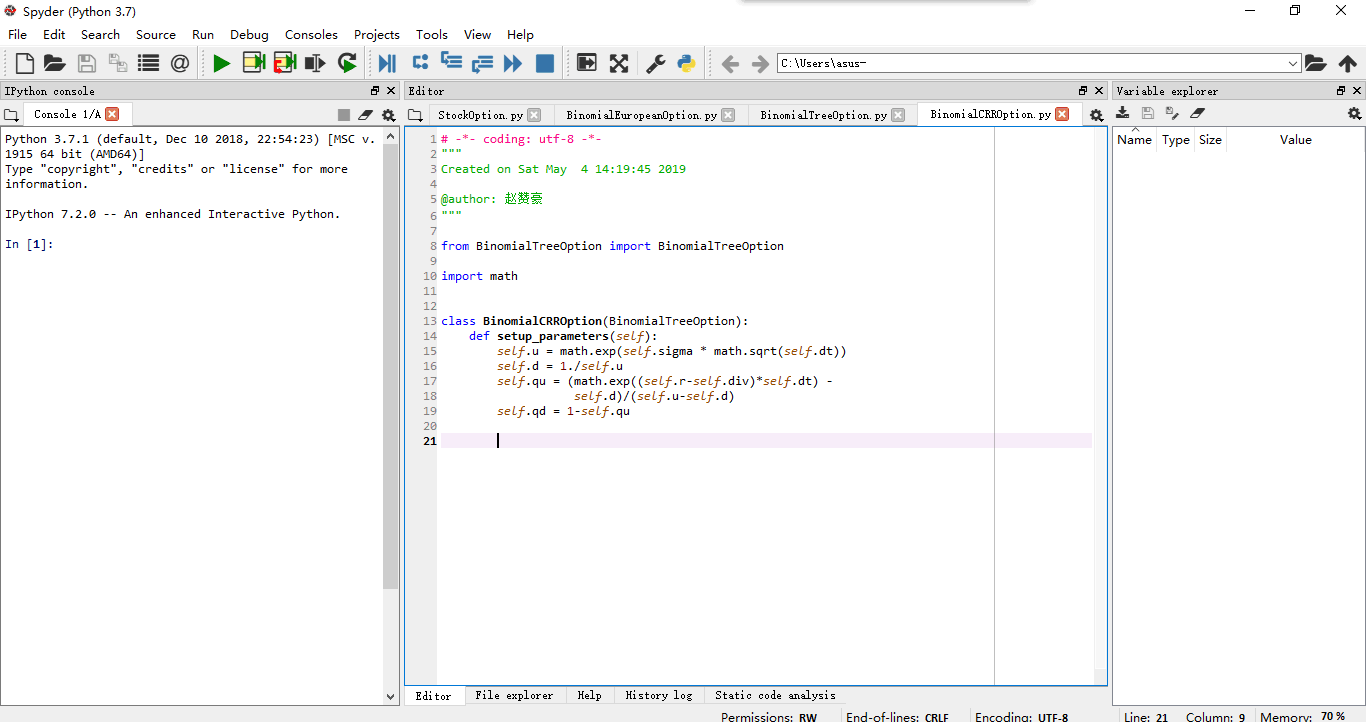
\includegraphics[height=5cm]{BinomialCRROption.png}
		\bicaption{BinomialCRROption类的编写 }{ }
		\label{fig:xfig1}
	\end{figure}



\subsection{Python实现二叉树定价模型}
	首先,我个人安装的是Python3.7.1+Anaconda3,在Anaconda3的集成环境中,有一个加Spyder的IDE。打开Spyder,然后打开工作目录下的StockOption.py,BinomialEuropeanOption.py,BinomialTreeOption.py,BinomialCRROption.py这四个.py文件。
	
	然后,依次运行StockOption.py,BinomialEuropeanOption.py,BinomialTreeOption.py,BinomialCRROption.py(按住F5即可运行)。运行结果如下图所示:
	
	\begin{figure}[htb] % use float package if you want it here
		\centering
		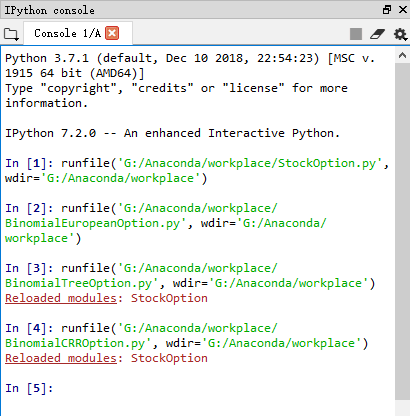
\includegraphics[height=5cm]{python1.png}
		\bicaption{Python依次运行编辑好的类文件}{ }
		\label{fig:xfig1}
	\end{figure}
	
	接下来,选用不同的类给期权进行定价。
	
	首先,给欧式看跌期权进行定价。假设在欧式看跌期权中,初始股价为50元,执行价格是52元,无风险利率是0.05,到期时间是2年,期数是2期,看涨的概率是0.2,看跌的概率是0.2。

	然后,给美式看跌期权定价。假设在美式看跌期权中,初始股价为50元,执行价格是52元,无风险利率是0.05,到期时间是2年,期数是2期,看涨的概率是0.2,看跌的概率是0.2。
	
	二叉树模型下的欧式看涨期权和美式看涨期权,得到的结果如下图:
	
	从下图中,可知,使用二叉树期权定价模型,得出欧式看跌期权的期权现值为4.1926542806038585元,得出美式看跌期权的期权现值为5.089632474198373元。
	\begin{figure}
		\begin{minipage}{0.48\textwidth}
			\centering
			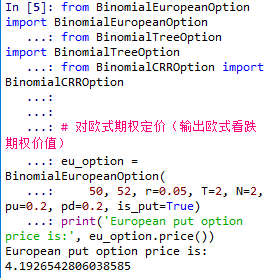
\includegraphics[height=5cm]{euoption.png}
			\caption{欧式看跌期权}
			\label{fig:parallel1}
		\end{minipage}\hfill
		\begin{minipage}{0.48\textwidth}
			\centering
			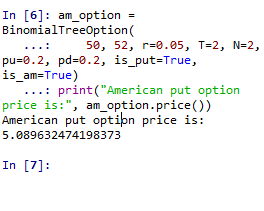
\includegraphics[height=5cm]{amoption.png}
			\caption{美式看跌期权}
			\label{fig:parallel2}
		\end{minipage}
	\end{figure}

	为什么同等条件下的欧式看跌期权和美式看跌期权的期权现值,美式看跌期权更高呢?因为美式期权可以在到期日前任意一天时点行权,欧式期权只能在到期日行权,因此美式期权的灵活性使得其价值不会低于对等的欧式期权的价值。
	
	若美式看涨期权的标的资产为不支付股息的股票,其对欧式看涨期权可能没有额外的价值。根据货币的时间价值理论,期权到期前行权比以相同行权价格在未来某个时间行权收益更小。对于不分配股息的实值美式看涨期权,期权持有人没有提前行权的动机。

	紧接着,使用CRR模型为欧式期权和美式期权进行定价。
	
	\begin{figure}[htb] % use float package if you want it here
		\centering
		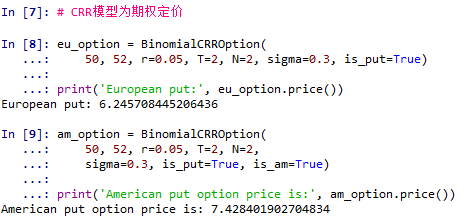
\includegraphics[height=5cm]{python2.png}
		\bicaption{CRR模型给期权定价}{ }
		\label{fig:xfig1}
	\end{figure}



%%%%%%%%%%%%%%%%% Black-Schools定价模型

\section{Black-Schools期权定价模型实现}

\subsection{R实现BS期权定价模型}
	在R中有个GBSOption函数可以间接的求出Black-Schools模型的定价结果。
	具体结果请看上述。
	
\subsection{SAS实现BS期权定价模型}
	SAS实现BS期权定价模型:
	
	\begin{figure}[htb] % use float package if you want it here
		\centering
		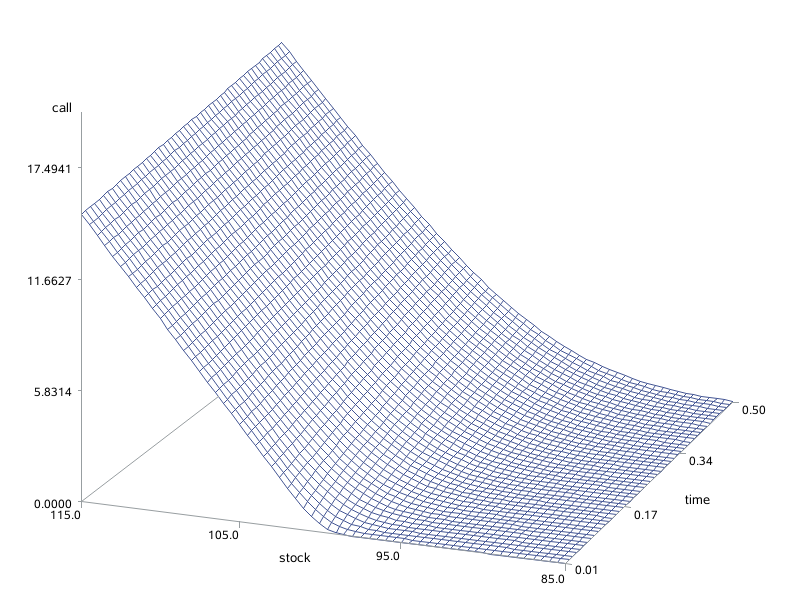
\includegraphics[height=5cm]{calloptionsas.png}
		\bicaption{欧式看涨期权价值的变动 }{ }
		\label{fig:xfig1}
	\end{figure}


	
	\begin{figure}[htb] % use float package if you want it here
		\centering
		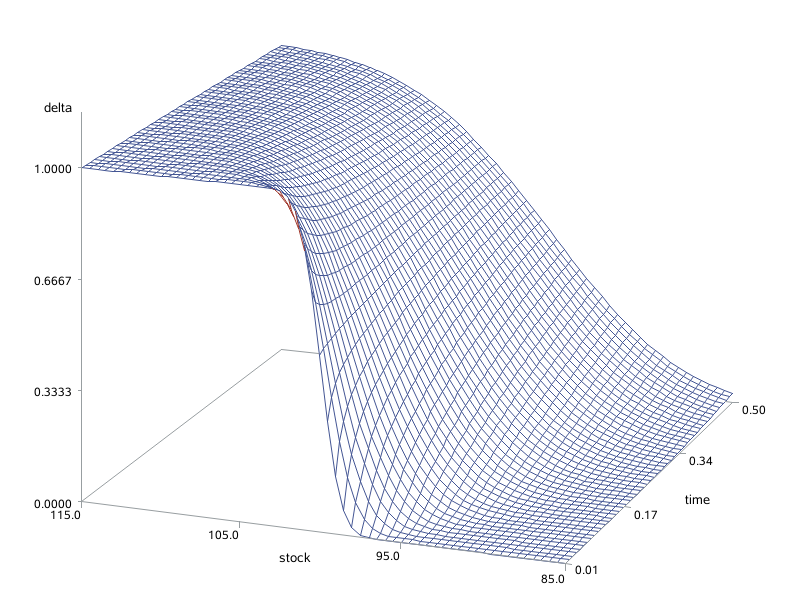
\includegraphics[height=5cm]{deltasas.png}
		\bicaption{欧式看涨期权的delta值随到期时间T、执行价格K的变化(SAS)}{ }
		\label{fig:xfig1}
	\end{figure}
	
	
	\begin{figure}[htb] % use float package if you want it here
		\centering
		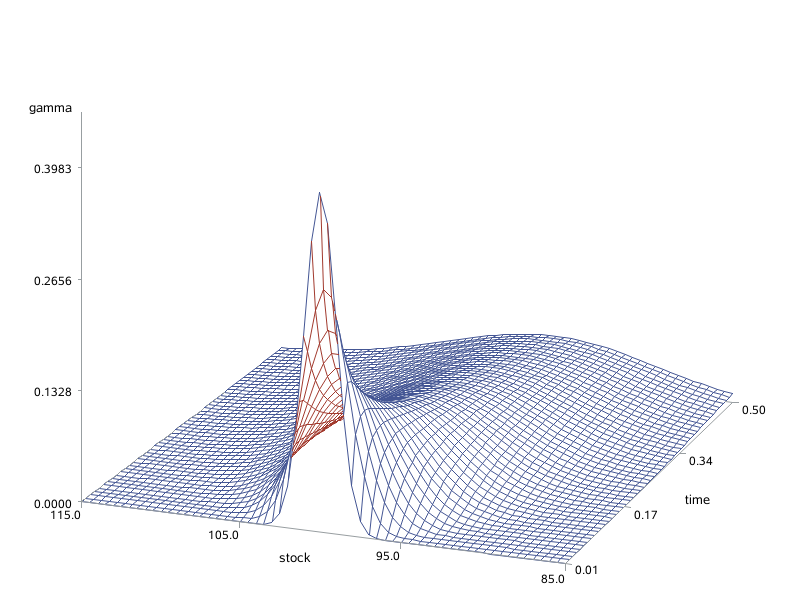
\includegraphics[height=5cm]{gammasas.png}
		\bicaption{欧式看涨期权的gamma值随到期时间T、执行价格K的变化}{ }
		\label{fig:xfig1}
	\end{figure}
	
		
	
	\begin{figure}[htb] % use float package if you want it here
		\centering
		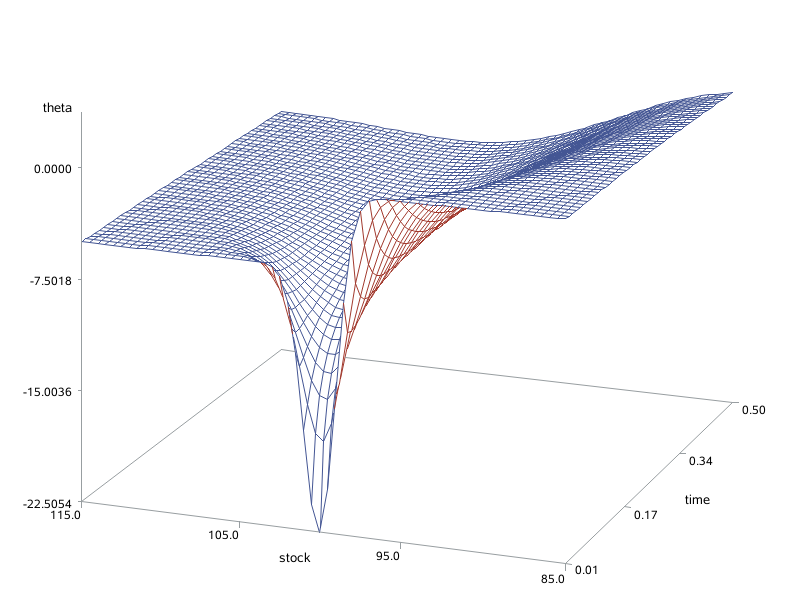
\includegraphics[height=5cm]{thetasas.png}
		\bicaption{欧式看涨期权的theta值随到期时间T、执行价格K的变化}{ }
		\label{fig:xfig1}
	\end{figure}
	
	
	
	
	
	\begin{figure}[htb] % use float package if you want it here
		\centering
		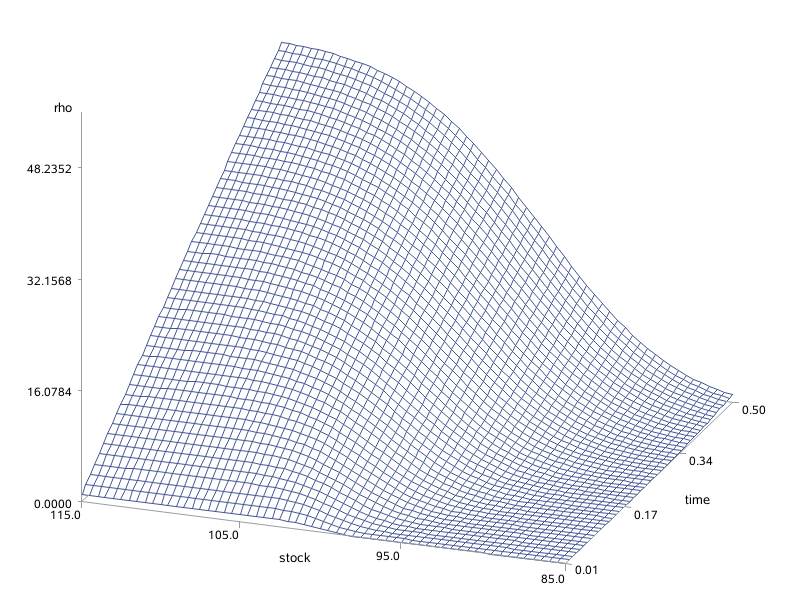
\includegraphics[height=5cm]{rhosas.png}
		\bicaption{欧式看涨期权的rho值随到期时间T、执行价格K的变化}{ }
		\label{fig:xfig1}
	\end{figure}
	
	
	
	
	\begin{figure}[htb] % use float package if you want it here
		\centering
		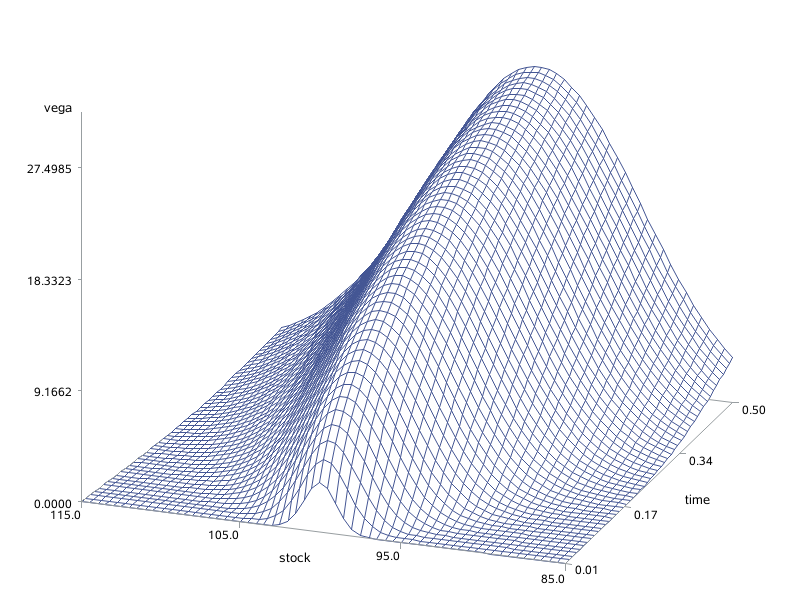
\includegraphics[height=5cm]{vegasas.png}
		\bicaption{欧式看涨期权的vega值随到期时间T、执行价格K的变化}{ }
		\label{fig:xfig1}
	\end{figure}
	
	
	
	
	
%%	强制换页
\clearpage		
\subsection{Python实现BS期权定价模型}
	自从Black,Scholes和Merton(BSM)在1973年发表了重要的论文后,BSM模型(连续市场模型)及相关的期权定价公式就被认为是期权定价的基准。其原因是,他们在一个简单但又具有一定现实意义的设定下提供了封闭解。两篇论文中推出的原始公式建立在两种不同的观点上。Black和Scholes提出的论点是均衡论点,他们认为一个无风险的资产组合在均衡收益,应该为无风险利率。Merton的论点则更为广泛地被应用,该论点认为(欧式)期权的价值应该等于能够完全复制该期权截止日期的收益,且具有适宜的交易策略的资产组合价值。

	几年后,Cox,Ross和Rubinstein(CRR)在1979年提出了二项式期权定价模型。该模型假定一个在离散时间和离散状态空间上的BSM经济体。BSM模型需要比较高深的数学,而且还需要求解偏微分方程,不过CRR分析只需要基本的概率论知识。直到今天,当很多人想用简单、直观的方法来讨论期权时,CRR用来代表不确定性的二叉树仍是重要的工具。而且,他们的数值方法不仅可以用于欧式期权定价,也可以很容易地用于美式期权定价。
	
	这两个市场模型的主要特征都是完全性:每个在未来时点到期的未定权益,都可以用两种可交易的资产——一个风险资产(比如指数或股票)和一个无风险债券的交易策略来复制。此外,当连续两期之间的时间间隔趋近于0时,CRR模型就会收敛为BSM模型。从这个角度来看,两个模型是一致的。

\subsubsection{Black-Scholes-Merton模型}
	在接下来的部分,我们主要研究欧式期权。所以,没有特别的说明,本节的“期权”就是欧式期权。为了更好地认识到期权价值对模型和期权参数的依赖情况,选取如下参数的期权作为案例来进行分析。
	
	\begin{enumerate}
		\item S$_{0}$=100:初始水平
		\item K=100:执行价格
		\item T=1.0:到期时间(年)
		\item r=0.05:无风险短期利率
		\item $\sigma$=0.2:指数的波动率
		\item t=0:定价日,即当期
	\end{enumerate}
	
	利用Python实现欧式看涨期权和看跌期权的定价公式,同时还包含了以上参数及看涨期权的图形输出,绘制的图形如下所示。以上参数和看跌期权的图形输出。每一个子图都只是改变一个基本参数得到的结果。
	
	
	
	\begin{figure}[htb] % use float package if you want it here
		\centering
		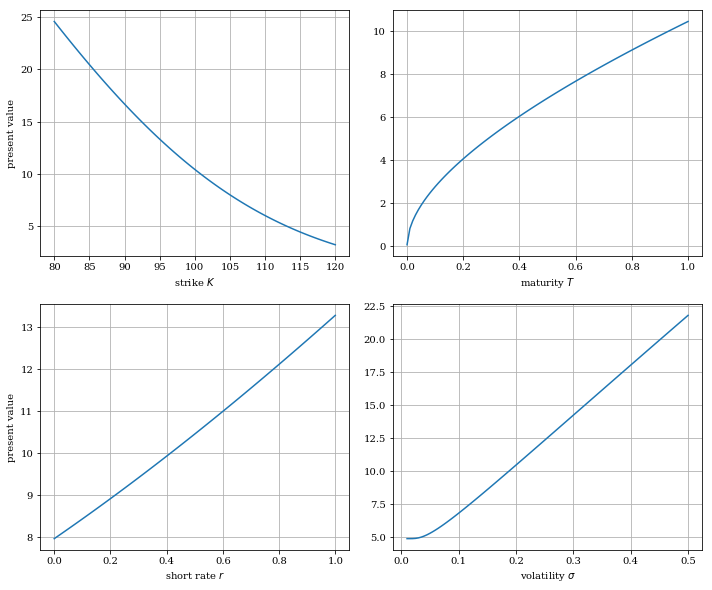
\includegraphics[height=5cm]{calloptionBS.png}
		\bicaption{欧式看涨期权价值随执行价格K、到期时间T、短期利率r、波动率$\sigma$的变动 }{ }
		\label{fig:xfig1}
	\end{figure}
	
	\begin{figure}[htb] % use float package if you want it here
		\centering
		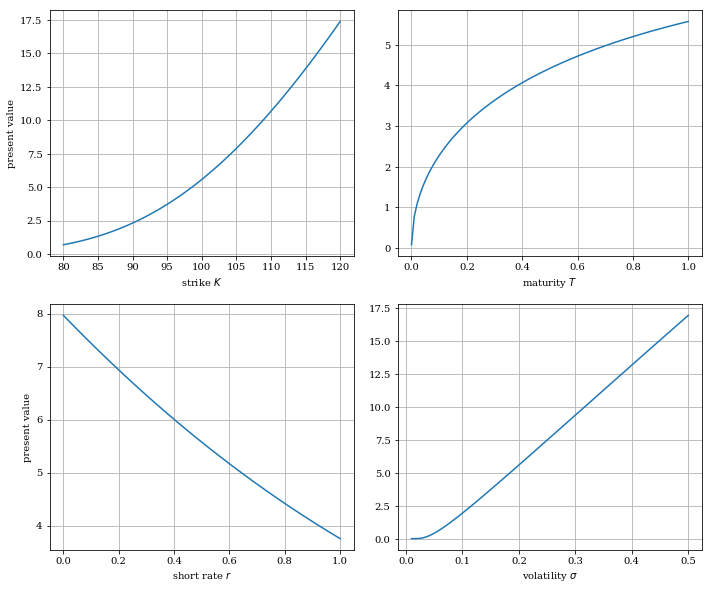
\includegraphics[height=5cm]{putoptionBS.png}
		\bicaption{欧式看跌期权价值随执行价格K、到期时间T、短期利率r、波动率$\sigma$的变动 }{ }
		\label{fig:xfig1}
	\end{figure}
	
	首先,价值状况进行比较。平价看涨期权($K=S_{0}=100,ATM$)的价值为10.4,远高于只值5.6的看跌期权,期权价内的程度越高(看涨期权:K<100;看跌期权:K>100,ITM),其价值也就越高。当期权价外的程度越高(看涨期权:K100;看跌期权:K<100,OTM),价值则越低。
	
	然后看到期时间,到期时间越长,期权的价值就越高。不过有的欧式期权并不是这样的,比如说深位价内欧式看涨期权。
	
	然后再看短期利率,短期利率的上升会增加看涨期权的价值,但是同时也会降低看跌期权的价值。在风险中性的条件下,指数随着短期利率的变动,而短期利率上涨越高对看涨期权就越有利,对看跌期权就越不利。
	
	最后看波动率,较高的波动率同时提高了看涨期权和看跌期权的价值,原因是两者在到期日变成价内的可能性都增加了。
	
	
	
	
	
	
	
\subsubsection{Black-Scholes-Merton模型的Greeks}
	
	
	
	\begin{figure}[htb] % use float package if you want it here
		\centering
		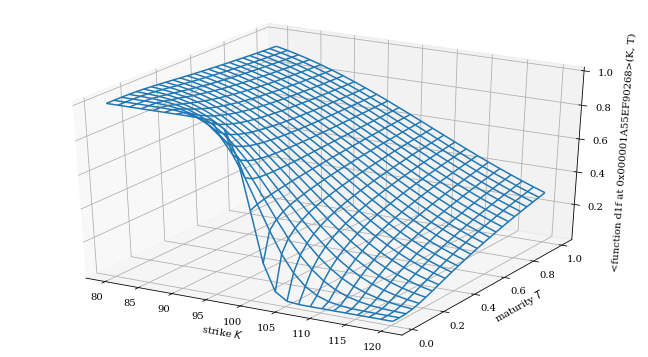
\includegraphics[height=5cm]{deltapy.png}
		\bicaption{欧式看涨期权的delta值随到期时间T、执行价格K的变化}{ }
		\label{fig:xfig1}
	\end{figure}
	
	
	
	
	
	\begin{figure}[htb] % use float package if you want it here
		\centering
		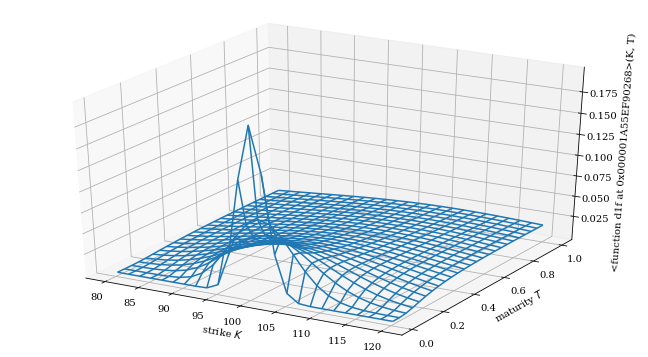
\includegraphics[height=5cm]{gammapy.png}
		\bicaption{欧式看涨期权的gamma值随到期时间T、执行价格K的变化}{ }
		\label{fig:xfig1}
	\end{figure}
	


	
	
	
	\begin{figure}[htb] % use float package if you want it here
		\centering
		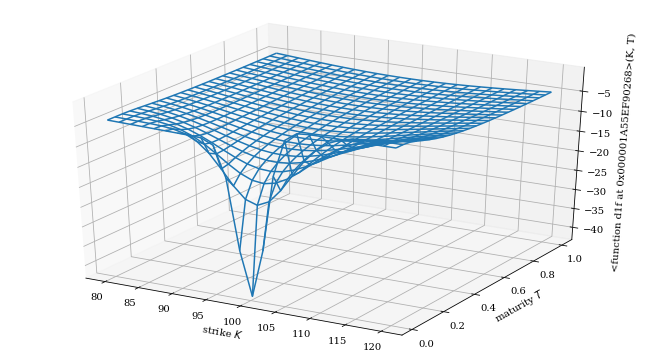
\includegraphics[height=5cm]{thetapy.png}
		\bicaption{欧式看涨期权的theta值随到期时间T、执行价格K的变化}{ }
		\label{fig:xfig1}
	\end{figure}





	\begin{figure}[htb] % use float package if you want it here
		\centering
		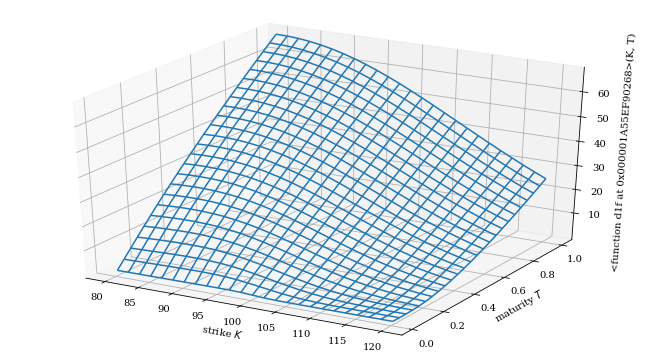
\includegraphics[height=5cm]{rhopy.png}
		\bicaption{欧式看涨期权的rho值随到期时间T、执行价格K的变化}{ }
		\label{fig:xfig1}
	\end{figure}




	\begin{figure}[htb] % use float package if you want it here
		\centering
		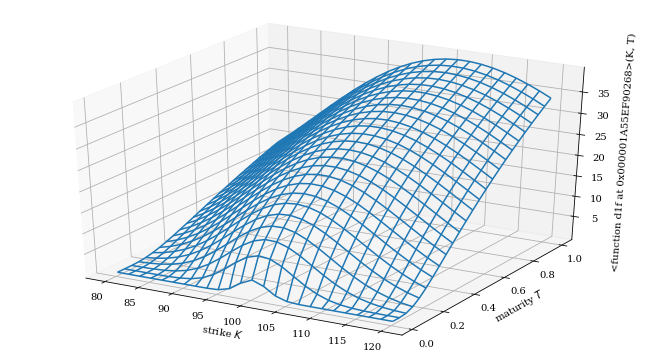
\includegraphics[height=5cm]{vegapy.png}
		\bicaption{欧式看涨期权的vega值随到期时间T、执行价格K的变化}{ }
		\label{fig:xfig1}
	\end{figure}
	
	
	
\section{蒙特卡罗期权定价模型实现}

\subsection{R实现蒙特卡罗期权定价模型}

\subsection{SAS实现蒙特卡罗期权定价模型}

\subsection{Python实现蒙特卡罗期权定价模型}










\chapter{基于大数据下二叉树期权定价实现}

\chapter{结果和分析}

\section{传统期权定价结果}

\section{基于大数据下期权定价结果}

\section{传统与大数据下期权定价的异同}

%% 结论
\chapter{结论}
\section{关于开发}\label{sec:dev}
本项目开源托管于Github,欢迎提交建议和意见,欢迎高质量的PR。项目地址为\url{https://github.com/nanmu42/CQUThesis}
\section{关于下载}
\begin{itemize}
	\item 发行版本,托管于CTAN,\url{https://www.ctan.org/pkg/cquthesis};
	\item 开发版本,位于Github,这个版本的更新最快,推荐使用。地址参见\ref{sec:dev}节。
\end{itemize}
\section{求助方案}
\begin{itemize}
	\item 在Github上提交Issue,地址:\url{https://github.com/nanmu42/cquthesis/issues}
	\item 加入重庆大学\TeX 用户组进行讨论,地址:\url{http://jq.qq.com/?_wv=1027&k=2HvYu95}
\end{itemize}
 
大家的反馈为模板提高带来机会。
\section{Happy Texing!}
祝你好运!



\chapter{具体命令}

\section{字体命令}\label{txt:FreqCmd}
{\kaishu 玲珑骰子安红豆,入骨相思知不知。\hfill ——温庭筠}
	
{\fangsong 愿得一心人,白头不相离。\hfill ——卓文君}
		
{\ifcsname youyuan\endcsname\youyuan\else[无 \cs{youyuan} 字体。]\fi 去年今日此门中,人面桃花相映红。\hfill ——崔护}
			
{\heiti 入我相思门,知我相思苦。\hfill ——李白}
				
{\ifcsname lishu\endcsname\lishu\else[无 \cs{lishu} 字体。]\fi 此情可待成追忆?只是当时已惘然。\hfill ——李商隐}
					
{\songti 雨打梨花深闭门,忘了青春,误了青春。\hfill ——唐寅}

使用\cs{textbf}和\cs{textit}以及\cs{underline}的效果分别如下:

这句话的\textbf{文字}分别\textit{使用}了三种命令来\underline{处理}。

The \textbf{words} in this sentences are \textit{processed} with three different \underline{cmd}.

\section{表格样本}

\subsection{基本表格}
\label{sec:basictable}

模板中关于表格的宏包有三个: \pkg{booktabs}、\pkg{array} 和\pkg{longtabular}。三线表可以用 \pkg{booktabs}提供的 \cs{toprule}、\cs{midrule} 和 \cs{bottomrule}。它们与\pkg{longtable} 能很好的配合使用。
\begin{table}[htb]
	\centering
	\begin{minipage}[t]{0.9\linewidth} % 如果想在表格中使用脚注,minipage是个不错的办法
	\caption[模板文件]{模板文件。如果表格的标题很长,那么在表格索引中就会很不美观,所以要像 chapter 那样在前面用中括号写一个简短的标题。这个标题会出现在索引中。}
	\label{tab:template-files}
	\begin{tabularx}{\linewidth}{lX}
		\toprule
		{\heiti 文件名} & {\heiti 描述} \\
		\midrule
		cquthesis.cls & 模板类文件\footnote{这是一个脚注}\\
		cquthesis.cfg & 模板配置文件\footnote{这是又一个脚注}\\
		cqunumberical.bst & 参考文献 BIB\TeX\ 样式文件。\\
		cquthesis.sty & 常用的包和命令写在这里,减轻主文件的负担。\footnote{同一页上的脚注最多支持到10个}\\
		\bottomrule
		\end{tabularx}
	\end{minipage}
\end{table}

首先来看一个最简单的表格。\autoref{tab:template-files} 列举了本模板主要文件及其功能。请大家注意三线表中各条线对应的命令。这个例子还展示了如何在表格中正确使用脚注。由于 \LaTeX{} 本身不支持在表格中使用\cs{footnote},所以我们不得不将表格放在小页中,而且最好将表格的宽度设置为小页的宽度,这样脚注看起来才更美观。

\subsection{双语题注和复杂表格}
\label{sec:complicatedtable}
使用\cs{bicaption}\marg{中文}\marg{英文}可以对图或者表的浮动体添加双语题注,对方程式进行双语题注,请使用\cs{eqlist}\marg{中文}\oarg{英文},注意括号。

我们经常会在表格下方标注数据来源,或者对表格里面的条目进行解释。前面的脚注是一种不错的方法,如果不喜欢脚注,可以在表格后面写注释,比如\autoref{tab:tabexamp1}。
\begin{table}[htbp]
	\centering
	\bicaption{复杂表格示例}{A more structured table}
	\label{tab:tabexamp1}
	\begin{minipage}[t]{0.8\textwidth} 
	\begin{tabularx}{\linewidth}{|l|X|X|X|X|}
		\hline
		\multirow{2}*{\diagbox[width=5em]{x}{y}} & \multicolumn{2}{c|}{First Half} & \multicolumn{2}{c|}{Second Half}\\\cline{2-5}
		& 1st Qtr &2nd Qtr&3rd Qtr&4th Qtr \\ \hline
		East$^{*}$ &   20.4&   27.4&   90&     20.4 \\
		West$^{**}$ &   30.6 &   38.6 &   34.6 &  31.6 \\ \hline
	\end{tabularx}\\[2pt]
	\footnotesize 
	*:东部\\
	**:西部
	\end{minipage}
\end{table}

此外,表~\ref{tab:tabexamp1} 同时还演示了另外两个功能:1)通过 \pkg{tabularx} 的\texttt{|X|} 扩展实现表格自动放大;2)通过命令 \cs{diagbox} 在表头部分插入反斜线。

\begin{table}[htbp]
	\noindent\begin{minipage}{0.5\textwidth}
		\centering
		\caption{第一个并排子表格}
		\label{tab:parallel1}
		\begin{tabular}{p{2cm}p{2cm}}
					\toprule
					No. & Name \\\midrule
					\xuhao[1] & Fox \\
					\xuhao & Panda \\
					\xuhao & Dog \\
					\bottomrule
		\end{tabular}
	\end{minipage}%
	\setxuhao[2]
	\begin{minipage}{0.5\textwidth}
		\centering
		\bicaption{第二个并排子表格}{The second subtable in one row}
		\label{tab:parallel2}
		\begin{tabular}{p{2cm}p{2cm}}
			\toprule
			No. & Name \\\midrule
			\xuhao[1] & Charlie \\
			\xuhao & Jack \\
			\xuhao & Tom \\
			\bottomrule
		\end{tabular}
	\end{minipage}
\end{table}

\begin{table}[htbp]
	\centering
	\caption{并排子表格}
	\label{tab:subtable}
	\subcaptionbox{第一个子表格}
	{
		\begin{tabular}{p{2cm}p{2cm}}
			\toprule
			111 & 222 \\\midrule
			222 & 333 \\\bottomrule
		\end{tabular}
	}
	\hskip2cm
	\subcaptionbox{第二个子表格}
	{
		\begin{tabular}{p{2cm}p{2cm}}
			\toprule
			111 & 222 \\\midrule
			222 & 333 \\\bottomrule
		\end{tabular}
	}
\end{table}

不可否认 \LaTeX{} 的表格功能没有想象中的那么强大,不过只要足够认真,足够细致,同样可以排出来非常复杂非常漂亮的表格。

\tabref{tab:parallel1}和\tabref{tab:parallel2}展示了\cs{xuhao}和\cs{xuhao}\texttt{[1]}的使用,可以达到自动编号的效果。不过要记得在每次使用之前使用\cs{resetxuhao},或者\cs{xuhao}\texttt{[1]}。使用\cs{setxuhao}\oarg{1-6}可以更改序号的标记方式,如\tabref{tab:parallel2}所示。详细用法请参阅用户手册。

\begin{longtable}[c]{c*{6}{r}}
	\bicaption[实验数据]{实验数据,这个题注是双语的,而且十分的长,注意这在索引中的处理方式}[Data in experiment]{Data in experiment, and this is a really long long long long long long long long long long text.}\label{tab:performance}\\
	\toprule
	测试程序 & \multicolumn{1}{c}{正常运行} & \multicolumn{1}{c}{同步} & \multicolumn{1}{c}{检查点} & \multicolumn{1}{c}{卷回恢复}
	& \multicolumn{1}{c}{进程迁移} & \multicolumn{1}{c}{检查点} \\
	& \multicolumn{1}{c}{时间 (s)}& \multicolumn{1}{c}{时间 (s)}&
	\multicolumn{1}{c}{时间 (s)}& \multicolumn{1}{c}{时间 (s)}& \multicolumn{1}{c}{
		时间 (s)}&  文件(KB)\\\midrule
	\endfirsthead
	\multicolumn{7}{c}{续表~\thetable\hskip1em 实验数据}\\
	\toprule
	测试程序 & \multicolumn{1}{c}{正常运行} & \multicolumn{1}{c}{同步} & \multicolumn{1}{c}{检查点} & \multicolumn{1}{c}{卷回恢复}
	& \multicolumn{1}{c}{进程迁移} & \multicolumn{1}{c}{检查点} \\
	& \multicolumn{1}{c}{时间 (s)}& \multicolumn{1}{c}{时间 (s)}&
	\multicolumn{1}{c}{时间 (s)}& \multicolumn{1}{c}{时间 (s)}& \multicolumn{1}{c}{
		时间 (s)}&  文件(KB)\\\midrule
	\endhead
	\hline
	\multicolumn{7}{r}{续下页}
	\endfoot
	\endlastfoot
	CG.A.2 & 23.05 & 0.002 & 0.116 & 0.035 & 0.589 & 32491 \\
	CG.A.4 & 15.06 & 0.003 & 0.067 & 0.021 & 0.351 & 18211 \\
	CG.A.8 & 13.38 & 0.004 & 0.072 & 0.023 & 0.210 & 9890 \\
	CG.B.2 & 867.45 & 0.002 & 0.864 & 0.232 & 3.256 & 228562 \\
	CG.B.4 & 501.61 & 0.003 & 0.438 & 0.136 & 2.075 & 123862 \\
	CG.B.8 & 384.65 & 0.004 & 0.457 & 0.108 & 1.235 & 63777 \\
	MG.A.2 & 112.27 & 0.002 & 0.846 & 0.237 & 3.930 & 236473 \\
	MG.A.4 & 59.84 & 0.003 & 0.442 & 0.128 & 2.070 & 123875 \\
	MG.A.8 & 31.38 & 0.003 & 0.476 & 0.114 & 1.041 & 60627 \\
	MG.B.2 & 526.28 & 0.002 & 0.821 & 0.238 & 4.176 & 236635 \\
	MG.B.4 & 280.11 & 0.003 & 0.432 & 0.130 & 1.706 & 123793 \\
	MG.B.8 & 148.29 & 0.003 & 0.442 & 0.116 & 0.893 & 60600 \\
	LU.A.2 & 2116.54 & 0.002 & 0.110 & 0.030 & 0.532 & 28754 \\
	LU.A.4 & 1102.50 & 0.002 & 0.069 & 0.017 & 0.255 & 14915 \\
	LU.A.8 & 574.47 & 0.003 & 0.067 & 0.016 & 0.192 & 8655 \\
	LU.B.2 & 9712.87 & 0.002 & 0.357 & 0.104 & 1.734 & 101975 \\
	LU.B.4 & 4757.80 & 0.003 & 0.190 & 0.056 & 0.808 & 53522 \\
	LU.B.8 & 2444.05 & 0.004 & 0.222 & 0.057 & 0.548 & 30134 \\
	CG.B.2 & 867.45 & 0.002 & 0.864 & 0.232 & 3.256 & 228562 \\
	CG.B.4 & 501.61 & 0.003 & 0.438 & 0.136 & 2.075 & 123862 \\
	CG.B.8 & 384.65 & 0.004 & 0.457 & 0.108 & 1.235 & 63777 \\
	MG.A.2 & 112.27 & 0.002 & 0.846 & 0.237 & 3.930 & 236473 \\
	MG.A.4 & 59.84 & 0.003 & 0.442 & 0.128 & 2.070 & 123875 \\
	MG.A.8 & 31.38 & 0.003 & 0.476 & 0.114 & 1.041 & 60627 \\
	MG.B.2 & 526.28 & 0.002 & 0.821 & 0.238 & 4.176 & 236635 \\
	MG.B.4 & 280.11 & 0.003 & 0.432 & 0.130 & 1.706 & 123793 \\
	MG.B.8 & 148.29 & 0.003 & 0.442 & 0.116 & 0.893 & 60600 \\
	LU.A.2 & 2116.54 & 0.002 & 0.110 & 0.030 & 0.532 & 28754 \\
	LU.A.4 & 1102.50 & 0.002 & 0.069 & 0.017 & 0.255 & 14915 \\
	LU.A.8 & 574.47 & 0.003 & 0.067 & 0.016 & 0.192 & 8655 \\
	LU.B.2 & 9712.87 & 0.002 & 0.357 & 0.104 & 1.734 & 101975 \\
	LU.B.4 & 4757.80 & 0.003 & 0.190 & 0.056 & 0.808 & 53522 \\
	LU.B.8 & 2444.05 & 0.004 & 0.222 & 0.057 & 0.548 & 30134 \\
	EP.A.2 & 123.81 & 0.002 & 0.010 & 0.003 & 0.074 & 1834 \\
	EP.A.4 & 61.92 & 0.003 & 0.011 & 0.004 & 0.073 & 1743 \\
	EP.A.8 & 31.06 & 0.004 & 0.017 & 0.005 & 0.073 & 1661 \\
	EP.B.2 & 495.49 & 0.001 & 0.009 & 0.003 & 0.196 & 2011 \\
	EP.B.4 & 247.69 & 0.002 & 0.012 & 0.004 & 0.122 & 1663 \\
	EP.B.8 & 126.74 & 0.003 & 0.017 & 0.005 & 0.083 & 1656 \\
	\bottomrule
\end{longtable}

如果你要排版的表格长度超过一页,那么推荐使用 \pkg{longtable} 或者 \pkg{supertabular}宏包,模板对 \pkg{longtable} 进行了相应的设置,所以用起来可能简单一些。表~\ref{tab:performance} 就是 \pkg{longtable} 的简单示例。

\section{定理环境}
\label{sec:theorem}

给大家演示一下各种和证明有关的环境:

\begin{assumption}
	假设以下数学方程成立:
	\begin{eqnarray}
	\label{eq:eqnxmp}
	c & = & a^2 - b^2\\
	& = & (a+b)(a-b)
	\end{eqnarray}
\end{assumption}

\begin{assumption}
	依然假设以下数学方程成立,注意整个系统是自动编号的:
	\begin{eqnarray}
	\label{eq:eqnxmp2}
	c & = & a^2 - b^2\\
	& = & (a+b)(a-b)
	\end{eqnarray}
\end{assumption}

\begin{definition}
	我们定义\ref{eq:eqnxmp}中的方程名称为\cquthesis 。你看,环境里是可以相互引用的。
\end{definition}

\begin{proposition}
	曾子曰:「吾日三省吾身 —— 为人谋而不忠乎?与朋友交而不信乎?传不习乎?」
\end{proposition}

多么凄美的命题啊!其日牛马嘶,新妇入青庐,奄奄黄昏后,寂寂人定初,我命绝今日,
魂去尸长留,揽裙脱丝履,举身赴清池,府吏闻此事,心知长别离,徘徊庭树下,自挂东南
枝。

\begin{remark}
	天不言自高,水不言自流。
	\begin{gather*}
	\begin{split} 
	\varphi(x,z)
	&=z-\gamma_{10}x-\gamma_{mn}x^mz^n\\
	&=z-Mr^{-1}x-Mr^{-(m+n)}x^mz^n
	\end{split}\\[6pt]
	\begin{align} \zeta^0&=(\xi^0)^2,\\
	\zeta^1 &=\xi^0\xi^1,\\
	\zeta^2 &=(\xi^1)^2,
	\end{align}
	\end{gather*}
\end{remark}

天尊地卑,乾坤定矣。卑高以陈,贵贱位矣。 动静有常,刚柔断矣。方以类聚,物以群分,
吉凶生矣。在天成象,在地成形,变化见矣。鼓之以雷霆,润之以风雨,日月运行,一寒一
暑,乾道成男,坤道成女。乾知大始,坤作成物。乾以易知,坤以简能。易则易知,简则易
从。易知则有亲,易从则有功。有亲则可久,有功则可大。可久则贤人之德,可大则贤人之
业。易简,而天下矣之理矣;天下之理得,而成位乎其中矣。

\begin{axiom}
	两点间直线段距离最短。  
	\begin{align}
	x&\equiv y+1\pmod{m^2}\\
	x&\equiv y+1\mod{m^2}\\
	x&\equiv y+1\pod{m^2}
	\end{align}
\end{axiom}

《彖曰》:大哉乾元,万物资始,乃统天。云行雨施,品物流形。大明始终,六位时成,时
乘六龙以御天。乾道变化,各正性命,保合大和,乃利贞。首出庶物,万国咸宁。

《象曰》:天行健,君子以自强不息。潜龙勿用,阳在下也。见龙再田,德施普也。终日乾
乾,反复道也。或跃在渊,进无咎也。飞龙在天,大人造也。亢龙有悔,盈不可久也。用九,
天德不可为首也。   

\begin{lemma}
	《猫和老鼠》是我最爱看的动画片。
	\begin{multline*}%\tag*{[a]} % 这个不出现在索引中
	\int_a^b\biggl\{\int_a^b[f(x)^2g(y)^2+f(y)^2g(x)^2]
	-2f(x)g(x)f(y)g(y)\,dx\biggr\}\,dy \\
	=\int_a^b\biggl\{g(y)^2\int_a^bf^2+f(y)^2
	\int_a^b g^2-2f(y)g(y)\int_a^b fg\biggr\}\,dy
	\end{multline*}
\end{lemma}

行行重行行,与君生别离。相去万余里,各在天一涯。道路阻且长,会面安可知。胡马依北
风,越鸟巢南枝。相去日已远,衣带日已缓。浮云蔽白日,游子不顾返。思君令人老,岁月
忽已晚。  弃捐勿复道,努力加餐饭。

\begin{theorem}\label{the:theorem1}
	犯我强汉者,虽远必诛\hfill —— 陈汤(汉)
\end{theorem}
\begin{subequations}
	\begin{align}
	y & = 1 \\
	y & = 0
	\end{align}
\end{subequations}
道可道,非常道。名可名,非常名。无名天地之始;有名万物之母。故常无,欲以观其妙;
常有,欲以观其徼。此两者,同出而异名,同谓之玄。玄之又玄,众妙之门。上善若水。水
善利万物而不争,处众人之所恶,故几于道。曲则全,枉则直,洼则盈,敝则新,少则多,
多则惑。人法地,地法天,天法道,道法自然。知人者智,自知者明。胜人者有力,自胜
者强。知足者富。强行者有志。不失其所者久。死而不亡者寿。

\begin{proof}
	燕赵古称多感慨悲歌之士。董生举进士,连不得志于有司,怀抱利器,郁郁适兹土,吾
	知其必有合也。董生勉乎哉?
	
	夫以子之不遇时,苟慕义强仁者,皆爱惜焉,矧燕、赵之士出乎其性者哉!然吾尝闻
	风俗与化移易,吾恶知其今不异于古所云邪?聊以吾子之行卜之也。董生勉乎哉?
	
	吾因子有所感矣。为我吊望诸君之墓,而观于其市,复有昔时屠狗者乎?为我谢
	曰:“明天子在上,可以出而仕矣!” \hfill —— 韩愈《送董邵南序》
\end{proof}

\begin{corollary}
	四川话配音的《猫和老鼠》是世界上最好看最好听最有趣的动画片。
	\begin{alignat}{3}
	V_i & =v_i - q_i v_j, & \qquad X_i & = x_i - q_i x_j,
	& \qquad U_i & = u_i,
	\qquad \text{for $i\ne j$;}\label{eq:B}\\
	V_j & = v_j, & \qquad X_j & = x_j,
	& \qquad U_j & u_j + \sum_{i\ne j} q_i u_i.
	\end{alignat}
\end{corollary}

迢迢牵牛星,皎皎河汉女。
纤纤擢素手,札札弄机杼。
终日不成章,泣涕零如雨。
河汉清且浅,相去复几许。
盈盈一水间,脉脉不得语。

\begin{example}
	大家来看这个例子。
	\begin{equation}
	\label{ktc}
	\left\{\begin{array}{l}
	\nabla f({\mbox{\boldmath $x$}}^*)-\sum\limits_{j=1}^p\lambda_j\nabla g_j({\mbox{\boldmath $x$}}^*)=0\\[0.3cm]
	\lambda_jg_j({\mbox{\boldmath $x$}}^*)=0,\quad j=1,2,\cdots,p\\[0.2cm]
	\lambda_j\ge 0,\quad j=1,2,\cdots,p.
	\end{array}\right.
	\end{equation}
\end{example}

\begin{exercise}
	清列出 Andrew S. Tanenbaum 和 W. Richard Stevens 的所有著作。
\end{exercise}

\begin{conjecture} \textit{Poincare Conjecture} If in a closed three-dimensional
	space, any closed curves can shrink to a point continuously, this space can be
	deformed to a sphere.
\end{conjecture}

\begin{problem}
	回答还是不回答,是个问题。 
\end{problem}

如何引用定理~\ref{the:theorem1} 呢?加上 \cs{label} 使用 \cs{ref} 即可。

\section{参考文献}
\label{sec:bib}
重庆大学的要求是参考文献以上标的形式标注于论述之后,就像这样:

研究表明\cite{r1},早睡早起有益身体健康。如果想同时引用多个文献\cite{r2,r3,r4,r6},只需要在\csgo{cite}{\null}中用逗号分开\textsf{citeKey}就好。

\cquthesis 同时提供正文模式的参考文献引用功能\cs{inlinecite},适用于以下情况:

文献\inlinecite{r6,z1,z2,z3}表明,文献\inlinecite{r7,r8,r9,r10}所述的情况是有理论依据的。

\section{数学公式}
\label{sec:equation}
贝叶斯公式如式~(\ref{equ:chap1:bayes}),其中 $p(y|\mathbf{x})$ 为后验;
$p(\mathbf{x})$ 为先验;分母 $p(\mathbf{x})$ 为归一化因子。
\begin{equation}
\label{equ:chap1:bayes}
p(y|\mathbf{x}) = \frac{p(\mathbf{x},y)}{p(\mathbf{x})}=
\frac{p(\mathbf{x}|y)p(y)}{p(\mathbf{x})} 
\end{equation}

论文里面公式越多,\TeX{} 就越 happy。再看一个 \pkg{amsmath} 的例子:
\newcommand{\envert}[1]{\left\lvert#1\right\rvert} 
\begin{equation}\label{detK2}
\det\mathbf{K}(t=1,t_1,\dots,t_n)=\sum_{I\in\mathbf{n}}(-1)^{\envert{I}}
\prod_{i\in I}t_i\prod_{j\in I}(D_j+\lambda_jt_j)\det\mathbf{A}
^{(\lambda)}(\overline{I}|\overline{I})=0.
\end{equation} 

前面定理示例部分列举了很多公式环境,可以说把常见的情况都覆盖了,大家在写公式的时候一定要好好看 \pkg{amsmath} 的文档,并参考模板中的用法:
\begin{multline*}%\tag{[b]} % 这个出现在索引中的
\int_a^b\biggl\{\int_a^b[f(x)^2g(y)^2+f(y)^2g(x)^2]
-2f(x)g(x)f(y)g(y)\,dx\biggr\}\,dy \\
=\int_a^b\biggl\{g(y)^2\int_a^bf^2+f(y)^2
\int_a^b g^2-2f(y)g(y)\int_a^b fg\biggr\}\,dy
\end{multline*}

这里还有一个多级规划公式,这个公式使用\csgo{listeq}{索引名}手动加入了目录后的索引。
\begin{equation}\label{bilevel}
\left\{\begin{array}{l}
\max\limits_{{\mbox{\footnotesize\boldmath $x$}}} F(x,y_1^*,y_2^*,\cdots,y_m^*)\\[0.2cm]
\mbox{subject to:}\\[0.1cm]
\qquad G(x)\le 0\\[0.1cm]
\qquad(y_1^*,y_2^*,\cdots,y_m^*)\mbox{ solves problems }(i=1,2,\cdots,m)\\[0.1cm]
\qquad\left\{\begin{array}{l}
\max\limits_{{\mbox{\footnotesize\boldmath $y_i$}}}f_i(x,y_1,y_2,\cdots,y_m)\\[0.2cm]
\mbox{subject to:}\\[0.1cm]
\qquad g_i(x,y_1,y_2,\cdots,y_m)\le 0.
\end{array}\right.
\end{array}\right.
\end{equation}\listeq{多级规划公式}
这些跟规划相关的公式都来自于清华大学刘宝碇老师《不确定规划》的课件。以上的许多例子由清华大学的薛瑞尼同学编写。

\section{化学方程式}

使用\pkg{mhchem}的\csgo{ce}{化学式或方程式}能够让你很容易地表示出各种化学式和化学方程:

例如:
\begin{center}
	\ce{C6H5-CHO}\\ \ce{A\bond{~--}B\bond{~=}C\bond{-~-}D}\\ \ce{SO4^2- + Ba^2+ -> BaSO4 v}
\end{center}

复杂一点的方程式也不在话下,如\eqref{eq:chem}:
\begin{equation}\label{eq:chem}
	\ce{Zn^2+
		<=>[+ 2OH-][+ 2H+]
		$\underset{\text{amphoteres Hydroxid}}{\ce{Zn(OH)2 v}}$ <=>[+ 2OH-][+ 2H+]
		$\underset{\text{Hydroxozikat}}{\ce{[Zn(OH)4]^2-}}$
	}
\end{equation}\eqlist{复杂的化学方程式}[A sophisticated chemical equation]

这个方程式嵌套在了\pkg{equation}环境中,可用\cs{eqlist}(\cs{listeq}的别名,作用相同)来编排到索引中。

如果你需要一次列举多个化学式,可以用\cs{cec}命令,例如,\csgo{cec}{H2O,HCl,CCl4}的输出为\cec{H2O,HCl,CCl4}。

\section{国际单位制(SI Unit)}

\cquthesis 采用\pkg{siunitx}作为国际单位制支持宏包,以下是一些使用例子,这个包的文档写得非常不错,请在命令行里输入\texttt{texdoc siunitx}察看。
\begin{center}
	\num{.3e45}\\
	\num{1.654 x 2.34 x 3.430}\\
	\si{\kilogram\metre\per\second}\\    
	\SIlist{0.13;0.67;0.80}{\milli\metre}
\end{center}


\section{绘图}
\label{sec:draw}

本模板不预先装载任何绘图包(如 \pkg{pstricks,pgf} 等),完全由用户来决定。个人觉得 \pkg{pgf} 不错,不依赖于 Postscript。此外还有很多针对 \LaTeX{} 的GUI 作图工具,如 XFig(jFig), WinFig, Tpx, Ipe, Dia, Inkscape, LaTeXPiX,jPicEdt, jaxdraw 等等。

\section{插图}
\label{sec:graphs}

推荐《\LaTeXe\ 插图指南》。关于子图形的使用细节请参看 \pkg{subcaption} 宏包的说明文档。

\subsection{一个图形}
\label{sec:onefig}
一般图形都是处在浮动环境中。之所以称为浮动是指最终排版效果图形的位置不一定与源文
件中的位置对应\footnote{这是\LaTeX 的一个设计特性。},这也是刚使
用 \LaTeX{} 同学可能遇到的问题。如果要强制固定浮动图形的位置,请使用 \pkg{float} 宏包,
它提供了 \texttt{[H]} 参数,比如图~\ref{fig:xfig1}。
\begin{figure}[htb] % use float package if you want it here
	\centering
	
\includegraphics[height=4cm]{CQUbadge.pdf}
	\bicaption{重庆大学校徽}{Chongqing University badage}
	\label{fig:xfig1}
\end{figure}

大学之道,在明明德,在亲民,在止于至善。知止而后有定;定而后能静;静而后能安;安
而后能虑;虑而后能得。物有本末,事有终始。知所先后,则近道矣。古之欲明明德于天
下者,先治其国;欲治其国者,先齐其家;欲齐其家者,先修其身;欲修其身者,先正其心;
欲正其心者,先诚其意;欲诚其意者,先致其知;致知在格物。物格而后知至;知至而后
意诚;意诚而后心正;心正而后身 修;身修而后家齐;家齐而后国治;国治而后天下
平。自天子以至于庶人,壹是皆以修身为本。其本乱而未治者 否矣。其所厚者薄,而其所
薄者厚,未之有也!

\hfill —— 《大学》


\subsection{多个图形}
\label{sec:multifig}

如果多个图形相互独立,并不共用一个图形计数器,那么用 \texttt{minipage} 或者\texttt{parbox} 就可以。否则,请参看
图~\ref{fig:big1-subcaptionbox},它包含两个小图,分别是图~\ref{fig:subfig1}和图~\ref{fig:subfig2}。推荐使用\cs{subcaptionbox},因为可以像图~\ref{fig:big1-subcaptionbox} 那样对齐子图的标题,也可以使用\pkg{subcaption}宏包的\cs{subcaption}(放在minipage中,用法同\cs{caption})或是\pkg{subfigure}、\pkg{subtable}环境,像图~\ref{fig:big1-subfigure},不要再用 \cs{subfloat}、\cs{subfigure} 和 \cs{subtable}。

\begin{figure}[h]
	\centering%
	\subcaptionbox{第一个小图形\label{fig:subfig1}}[3cm] %标题的长度,超过则会换行,如下一个小图。
	{
\includegraphics[height=4cm]{CQUbadge.pdf}}%
	\hspace{4em}%
	\subcaptionbox{第二个小图形,注意这个图略矮些。如果标题很长的话,它会自动换行\label{fig:subfig2}}
	{
\includegraphics[height=3cm]{CQUbadge.pdf}}
	\caption{包含子图形的大图形(subcaptionbox示例)}
	\label{fig:big1-subcaptionbox}
\end{figure}
\begin{figure}[ht]
	\centering%
	\begin{subfigure}{3cm}
		
\includegraphics[height=4cm]{CQUbadge.pdf}
		\caption{第一个小图形}
	\end{subfigure}%
	\hspace{4em}%
	\begin{subfigure}{0.5\textwidth}
		
\includegraphics[height=3cm]{CQUbadge.pdf}
		\caption{第二个小图形,注意这个图略矮些。subfigure中同一行的子图在顶端对齐。}
	\end{subfigure}
	\caption{包含子图形的大图形(subfigure示例)}
	\label{fig:big1-subfigure}
\end{figure}

如果要把编号的两个图形并排,那么小页就非常有用了。
\begin{figure}
	\begin{minipage}{0.48\textwidth}
		\centering
		
\includegraphics[height=5cm]{CQUbadge.pdf}
		\caption{并排第一个图}
		\label{fig:parallel1}
	\end{minipage}\hfill
	\begin{minipage}{0.48\textwidth}
		\centering
		
\includegraphics[height=5cm]{CQUbadge.pdf}
		\caption{并排第二个图}
		\label{fig:parallel2}
	\end{minipage}
\end{figure}

测试用途:theequation值为:\theequation ,thefigure值为:\thefigure ,thetable值为:\thetable




\backmatter %%% 后置部分(致谢、参考文献、附录等)





%% 致谢

\chapter{致\hskip\ccwd{}谢}

% 这里用盲审环境包裹致谢,在开启盲审开关时,环境内部的内容不予渲染。
\begin{secretizeEnv}
	这篇文章是我在重庆理工大学学习的本科毕业论文。感谢一直以来支持我的家人、女朋友、老师、朋友、同学对我的支持!在这里,我由衷地感谢肖枝洪老师对我的培养。肖老师是我的大学时代的SAS课程的任课老师,他的认真负责让我印象深刻!
	
	初识肖枝洪老师是在我们专业的培养计划课上,当时我还不太了解自己专业是干嘛的。日后相处,我惊讶于肖老师对统计知识的精湛诠释,又深深地感召于肖老师的独特的人格魅力。近四年来,肖老师言传身教,传道授业,让我受益匪浅!
		
	感谢吕贵臣、唐朝君等任课老师,是您们严谨的教学态度,让我打下了坚实的数学基础!
	
	感谢洪雄老师,您讲授C语言课程幽默风趣,您是我编程的启蒙老师,感谢您!
	
	感谢朱小飞老师,您讲授的MATLAB课程让我对编程语言有了更多的理解,感谢您!
	
	感谢卢鹏老师、张松林老师、张露老师、曾雪老师对我大学四年的教导,非常感谢您们!
	
	最后,我想感谢我的女朋友,谢谢你一直以来对我的帮助和支持!
	
\end{secretizeEnv}








%% 参考文献
% 顺序编码制:cqunumerical		
% 注意:至少需要引用一篇参考文献,否则下面两行会引起编译错误。
%\bibliographystyle{cqunumerical}
%\bibliography{ref/refs}

%% 自己添加参考文献的方式




\begin{thebibliography}{1}
	\addcontentsline{toc}{section}{参考文献}
	\bibitem{cox}  Cox, J. C., J. E. Ingersoll, and S. A. Ross. An Intertemporal General Equilibrium Model of Asset Prices, Econometrica, 53(1985), 363-84.
	\bibitem{cox} Cox, J. C., S. A. Ross, and M. Rubinstein. Option Pricing: A Simplified Approach, Journal of Financial Economics, 7(October 1979), 229-64.
	\bibitem{cox} Cox, J. C., and M. Rubinstein. Option Markets. Englewood Cliffs, N. J.: Prentice Hall,1985.
	\bibitem{cox} Cox, J. C., S. A. Ross. The Valuation of Options for Alternative Stochastic Processes, Journal of Financial Economics, 3(1976), 145-66.
	\bibitem{black} Black, F. Fact and Fantasy in the Use of Options and Corporate Liabilities, Financial Analysts Journal, 31(July-August 1975), 36-41, 61-42.
	\bibitem{black} Black, F., and M. Scholes. The Valuation of Option Contracts and a Test of Market Efficiency, Journal of Finance, 27(May 1972), 399-418.
	\bibitem{black} Black, F., and M. Scholes. The Pricing of Options and Corporate Liabilities. Journal of Political Economy. 81(May-June 1973), 637-59.
	\bibitem{liu} 刘海洋. \LaTeX 入门 [M]. 北京: 电子工业出版社, 2013.
	\bibitem{hu}  胡伟. \LaTeX 2e完全学习手册(第二版)[M] 北京: 清华大学出版社, 2013.
	\bibitem{zhu}  朱世武.金融计算与建模理论、算法与SAS程序[M].北京:清华大学出版社,2007.
	\bibitem{xu}  许启发,蒋翠侠.R软件及其在金融定价分析中的应用[M].北京:清华大学出版社,2015.
	\bibitem{song}  宋军,张宗新.金融计量学-基于SAS的金融实证研究[M].北京:北京大学出版社,2009.
	\bibitem{cai}   (美)蔡瑞胸;王远林,王辉,潘家栋译.金融时间序列分析(第三版)[M].北京:人民大学出版社,2012.
	\bibitem{wu}  吴喜之.复杂数据的统计方法-基于R的应用(第二版)[M].北京:中国人民大学出版社,2013.
	\bibitem{ma}  (新) 马伟民;张永冀,霍达,张彤译.Python金融数据分析[M].北京:机械工业出版社,2018.
\end{thebibliography}








%% 附录(按ABC...分节,证明、推导、程序、个人简历等)
\appendix

% 个人简历

\chapter{附\hskip\ccwd{}录}


\section{程序源代码}

R实现多期二叉树:
\begin{lstlisting}
# 实现二叉树定价

# 安装fOptions包
#install.packages("fOptions")
#install.packages("timeDate")
#install.packages("timeSeries")
#install.packages("fBasics")

# 加载fOptions包
library(timeDate)
library(timeSeries)
library(fBasics)
library(fOptions)

CRRBinomialTreeOption(TypeFlag='ce', S=100, X=110,
 Time=6/12, r=0.05, b=0.05, sigma=0.2, n=3,
 title="二叉树定价")

# BS模型定价
GBSOption(TypeFlag = 'c', S=100, X=110, Time=6/12, r=0.05, 
b=0.05, sigma = 0.2, title="Black-Schools定价" )@price


# 实现3期二叉树定价
CRRTree=BinomialTreeOption(TypeFlag = 'pa', S=100, X=110, 
Time=6/12, r=0.05, b=0.05, sigma=0.2, n=3)

BinomialTreePlot(CRRTree, dy=1, cex=0.8, ylim=c(-5,5), 
xlab='n期', ylab='期权价值', main='选择树')


# 实现20期二叉树定价
CRRTree=BinomialTreeOption(TypeFlag = 'pa', S=100, X=110, 
Time=6/12, r=0.05, b=0.05, sigma=0.2, n=20)

BinomialTreePlot(CRRTree, dy=1, cex=0.8, ylim=c(-22,22), 
xlab='n期', ylab='期权价值', main='选择树')
\end{lstlisting}


SAS实现多期二叉树:
\begin{lstlisting}	
proc iml;
/* 看涨期权的定价公式 */
start call(i,sigma,t,S,X,n);
R=exp(i*t/n);
u=exp(sigma*sqrt(t/n));
d=exp(-sigma*sqrt(t/n));
q=(r-d)/(u-d);
index=(n:0);
matrix=j(n+1,3,.);
do i=1 to n+1;
matrix[i,1]=comb(n,index[i]);
matrix[i,2]=q**index[i]*(1-q)**(n-index[i]);
matrix[i,3]=max(S*u**index[i]*d**(n-index[i])-X,0);
end;
c=matrix[,#][+,] / R ** n;
return(c);
finish call;

/* 看跌期权的定价公式 */
start put(i,sigma,t,S,X,n);
R=exp(i*t/n);
u=exp( sigma * sqrt(t/n) );
d=exp(-sigma * sqrt(t/n) );
q=(r-d) / (u-d);
index=(n:0);
matrix=j(n+1,3,.);
do i=1 to n+1;
matrix[i,1]=comb(n,index[i]);
matrix[i,2]=q**index[i]*(1-q)**(n-index[i]);
matrix[i,3]=max(X-S*u**index[i]*d**(n-index[i]),0);
end;
p=matrix[,#][+,] / R ** n;
return(p);
finish put;

/* 调整n的大小,并计算看涨期权和看跌期权 */
do n=5 to 1000 by 5;
call=j(nrow(n),1,.);
put=j(nrow(n),1,.);
mattrib call format=5.3 put format=5.3;
do k=1 to nrow(n);
call[k]=round(call(0.05,0.1,1,100,100,n[k]),0.001);
put[k]=round(put(0.05,0.1,1,100,100,n[k]),0.001);
end;
print n call put;
end;

/* 调整i的大小,并计算看涨期权和看跌期权 */
do i=0.002 to 0.1 by 0.002;
call=j(nrow(i),1,.);
put=j(nrow(i),1,.);
mattrib i format=percent7.1 call format=5.3
 put format=5.3;
do k=1 to nrow(i);
call[k]=round(call(i[k],0.1,1,100,100,1000),0.001);
put[k]=round(put(i[k],0.1,1,100,100,1000),0.001);
end;
print i call put;
end;

/* 调整sigma的大小,并计算看涨期权和看跌期权 */
do sigma=0.01 to 0.5 by 0.01;
call=j(nrow(sigma),1,.);
put=j(nrow(sigma),1,.);
mattrib sigma format=percent7.1 call format=5.3 
put format=5.3;
do k=1 to nrow(sigma);
call[k]=round(call(0.05,sigma[k],1,100,100,1000),0.001);
put[k]=round(put(0.05,sigma[k],1,100,100,1000),0.001);
end;
print sigma call put;
end;

/* 调整t的大小,并计算看涨期权和看跌期权 */
do t=0.1 to 5 by 0.1;
call=j(nrow(t),1,.);
put=j(nrow(t),1,.);
mattrib t format=5.1 call format=5.3 put format=5.3;
do k=1 to nrow(t);
call[k]=round(call(0.05,0.1,t[k],100,100,1000),0.001);
put[k]=round(put(0.05,0.1,t[k],100,100,1000),0.001);
end;
print t call put;
end;

/* 调整x的大小,并计算看涨期权和看跌期权 */
do x=80 to 130 by 1;
call=j(nrow(x),1,.);
put=j(nrow(x),1,.);
mattrib x format=5.1 call format=5.3 put format=5.3;
do k=1 to nrow(x);
call[k]=round(call(0.05,0.1,1,100,x[k],1000),0.001);
put[k]=round(put(0.05,0.1,1,100,x[k],1000),0.001);
end;
print x call put;
end;
quit;
\end{lstlisting}

Python编写StockOption类:
\begin{Python}
	
	# -*- coding: utf-8 -*-
	"""
	Created on Fri May  3 10:08:18 2019
	
	@author: 赵赞豪
	"""
	
	# 编写StockOption类
	import math
	
	class StockOption(object):
	def __init__(self, S0, K, r, T, N, params):
	self.S0 = S0
	self.K  = K
	self.r  = r
	self.T  = T
	self.N  = max(1, N)
	self.STs= None
	
	self.pu          = params.get("pu", 0)
	self.pd          = params.get("pd", 0)
	self.div         = params.get("div", 0)
	self.sigma       = params.get("sigma", 0)
	self.is_call     = params.get("is_call", True)
	self.is_european = params.get("is_eu", True)
	
	self.dt = T/float(N)
	self.df = math.exp(-(r-self.div)*self.dt)
		
\end{Python}


Python编写BinomialEuropeanOption类:
\begin{Python}
	# -*- coding: utf-8 -*-
	"""
	Created on Fri May  3 10:46:08 2019
	
	@author: 赵赞豪
	"""
	
	
	from StockOption import StockOption
	import math
	import numpy as np
	
	class BinomialEuropeanOption(StockOption):
	def __setup_parameters__(self):
	self.M  = self.N + 1
	self.u  = 1 + self.pu
	self.d  = 1 - self.pd
	self.qu = (math.exp((self.r-self.div)*self.dt) - self.d) / (self.u-self.d)
	self.qd = 1-self.qu
	
	def _initialize_stock_price_tree_(self):
	self.STs = np.zeros(self.M)
	for i in range(self.M):
	self.STs[i] = self.S0*(self.u**(self.N-i))*(self.d**i)
	
	def _initialize_payoffs_tree_(self):
	payoffs = np.maximum(0, (self.STs - self.K) if self.is_call else (self.K - self.STs))
	return payoffs
	
	def _traverse_tree_(self, payoffs):
	for i in range(self.N):
	payoffs = (payoffs[:-1] * self.qu + payoffs[1:] * self.qd) * self.df
	return payoffs
	
	def __begin_tree_traversal__(self):
	payoffs = self._initialize_payoffs_tree_()
	return self._traverse_tree_(payoffs)
	
	def price(self):
	self.__setup_parameters__()
	self._initialize_stock_price_tree_()
	payoffs = self.__begin_tree_traversal__()
	return payoffs[0]
\end{Python}


















\section{附录的图和表}
以下内容用来测试附录中的插图和插表是否正常,主要的关注点在题注:

\begin{figure}[tbh]
\centering

\includegraphics[width=0.5\linewidth]{CQUbadge}
\caption{附录插图测试}
\label{fig:cqubadge}
\end{figure}

\begin{figure}[tbh]
	\centering
	
\includegraphics[width=0.5\linewidth]{CQUbadge}
	\caption{附录插图测试}
	\label{fig:cqubadge2}
\end{figure}

\begin{table}[htb]
	\centering\colsep[24pt]
	\caption{本课题研究的两个自变量}
	\label{tab:inroVarible}
	\begin{tabularx}{\linewidth}{cl}
		\toprule
		\headcell{自变量} & \headcell{自变量可取的值} \\
		\midrule\setxuhao[6]
		是否接触大气 & \xuhao[1] 接触大气 \xuhao 氮气保护 \\\setxuhao[2]
		溶解方式 & \xuhao[1] 超声30min \xuhao 搅拌1h \xuhao 静置12h\\
		表格的第三行 & \bigcell{使用\cs{bigcell}\\可主动换行}\\
		\bottomrule
	\end{tabularx}
\end{table}

\begin{equation}
\alpha\beta\gamma\delta\epsilon\varepsilon\zeta\eta = AB\Gamma\varGamma Z
\end{equation}\eqlist{附录中的公式编号1,双语}[Equation name in English A]

\begin{equation}
\alpha\beta\gamma\delta\epsilon\varepsilon\zeta\eta = CD\Gamma\varGamma Z
\end{equation}\eqlist{附录中的公式编号2,双语}[Equation name in English B]

测试用途:theequation值为:\theequation ,thefigure值为:\thefigure ,thetable值为:\thetable

%% 原创声明和授权说明书,可选:用扫描页替换
%\cquauthpage[contents/authscan.pdf]

% 注释掉没有用的页面
%\cquauthpage

\end{document}
